\documentclass{article}
\usepackage{graphicx}
\usepackage{amsfonts}
\usepackage{tabularx}
\usepackage{xcolor}
\usepackage{listings}
\usepackage{proof}
\usepackage[T1]{fontenc}
\usepackage{textcomp}
\usepackage{amsmath}
\usepackage{bbm}
\usepackage{hyperref}
\usepackage{amssymb}
\hypersetup{
    colorlinks,
    citecolor=black,
    filecolor=black,
    linkcolor=black,
    urlcolor=black
}

\lstset{
 language=caml,
 columns=[c]fixed,
% basicstyle=\small\ttfamily,
 keywordstyle=\bfseries,
 upquote=true,
 commentstyle=,
 breaklines=true,
 showstringspaces=false,
 stringstyle=\color{blue},
 literate={'"'}{\textquotesingle "\textquotesingle}3
}

\title{Appunti Fondamenti Logici per l'informatica}
\author{Gabriele Genovese}
\date{\today}

\begin{document}

\maketitle

\tableofcontents

\newpage

\section{Primo modulo: $\lambda$-Calcolo}

\subsection{Formalismo di calcolo}
Un formalismo di calcolo è un formalismo che risponde alla domanda “cosa vuol dire calcolare”.

\subsubsection{Formalismo}
Un formalismo è una descrizione matematicamente rigorosa di un fenomeno, in genere ottenuta tramite manipolazione di espressioni simboliche.
        
\subsubsection{Esempi formalismi di calcolo}
$\lambda$-calcolo, macchine di Turing, sistemi di Post, funzioni primitive ricorsive con operatore di minimizzazione, Random Access Machines, linguaggi di programmazione rigorosamente specificati, etc\ldots
     
\subsection{Tesi di Church-Turing}   
Tesi intesa come congettura, perché è impossibile da dimostrare.
\begin{quote}
Ogni funzione calcolabile da un formalismo di calcolo sufficientemente espressivo è calcolabile da una macchina di Turing e viceversa.
\end{quote}
Tutti i formalismi sono equivalenti dal punto di vista di cosa calcolano. Formalismi diversi hanno punti di forza/debolezza diversi (come i linguaggi di programmazione).
    
\subsection{Macchine di Turing contro $\lambda$-calcolo}
Nelle macchine di Turing ``calcolare" significa modificare un supporto fisico di celle discrete, ognuna contenente una quantità finita di informazione. Il Calcolo è ottenuto tramite operazioni locali (una testina r/w si muove sul supporto fisico). Oltre al supporto fisico, la macchina è in uno stato scelto da un insieme finito.

\bigskip

Nel $\lambda$-calcolo ``calcolare" significa semplificare delle espressioni. Le espressioni sono funzioni. In particolare, le funzioni prendono in input funzioni e danno in output funzioni.

\begin{table}[!ht]
    \centering
    \begin{tabularx}{\textwidth}{|X|X|}
        \hline
        \textbf{Macchine di Turing} & \textbf{$\lambda$-calcolo}  \\ \hline
        Ogni passo $O(1)$ (tempo) & Implementazione naif di un passo: $O(n^2)$  \\ \hline
        Ogni cella $O(1)$ (spazio) & Implementazione efficiente: $O(???)$   \\ \hline
        Ottimo per lo studio della complessità & Pessimo per lo studio della complessità \\ \hline
    \end{tabularx}
    \caption{Differenze riguardanti la complessità}
    \label{tab:turvslam-compl}
\end{table}

\begin{table}[!ht]
    \centering
    \begin{tabularx}{\textwidth}{|X|X|}
        \hline
        \textbf{Macchine di Turing} & \textbf{$\lambda$-calcolo}  \\ \hline
        Imperativo, ma $\not =$ dai linguaggi imperativi & Cuore di tutti i linguaggi funzionali  \\ \hline
        Non composizionale & Composizionale \\ \hline
        Basso livello & Alto livello  \\ \hline
        Difficile implementare costrutti/dati/meccanismi & Facile implementare costrutti/dati/meccanismi  \\ \hline
        Definizione non ricorsiva, quindi fare prove formali è complesso & Definizioni ricorsiva, quindi fare prove formali è facile per induzione \\ \hline
        Pessimo per lo studio dei linguaggi di programmazione & Ottimo per lo studio dei linguaggi di programmazione \\ \hline
        Ad-hoc & Controparte computazionale della logica \\ \hline
    \end{tabularx}
    \caption{Differenze riguardanti le caratteristiche}
    \label{tab:turvslam-ling}
\end{table}

\pagebreak

\subsection{Macchine di Turing}    
Una macchina di Turing è definita da una tupla $(A, Q, q_0, q_f, \delta)$ dove:
\begin{itemize}
    \item L’alfabeto $A$ è un insieme non vuoto, finito di simboli
    \item L’insieme di stati $Q$ è un insieme non vuoto, finito di stati
    \item $q_0\in Q$ è lo stato iniziale
    \item $q_f \in Q$ è lo stato finale
    \item La funzione di transizione $\delta$ ha dominio $A \to Q$ e codominio $A \to Q \to \{L, R\}$
\end{itemize}

\subsubsection{Stato di una macchina di Turing}
Lo stato di una macchina di Turing $(A, Q, q_0, q_f,\delta )$ è una tripla $(\alpha, i , q)$ dove:
\begin{itemize}
    \item Il nastro infinito $\alpha$ è una funzione da $\mathbb{Z}$ a $A$ \\ Intuizione: $\alpha(k) = a$ sse la $k$-esima cella del nastro contiene il simbolo $a$
    \item  $i \in \mathbb{Z}$ è la posizione della testina sul nastro \\ Intuizione: la testina è posizionata sulla $i$-esima cella di contenuto $\alpha(i)$
    \item $q \in Q$ è lo stato corrente
\end{itemize}

Uno stato $(\alpha, i, q)$ è iniziale di input $\alpha$ sse $i = 0$ e $q = q_0$ e finale di output $\alpha$ sse $q = q_f$.

\subsubsection{Esecuzione di una macchina di Turing}
Una macchina di Turing $(A, Q, q_0, q_f,\delta )$ in uno stato $(\alpha, i , q)$ non finale {\color{red}transisce} in un nuovo stato $(\alpha', i', q')$ se:
\begin{itemize}
    \item $\delta(\alpha(i), q) = a, q', x$ \\ Intuizione: la testina {\color{red} legge} il contenuto $\alpha(i)$ della cella corrente $i$, lo stato corrente {\color{red} si aggiorna} da $q$ a $q'$ e ...
    \item $\alpha'(i) = a$ e $\alpha'(n)=\alpha(n)$ per $n\not = i$\\ ... la testina {\color{red} sovrascrive} il valore della cella con $a$ e ...
    \item $i' = i+1$ se $x = R; i' = i-1$ se $x = L$ \\ ... {\color{red} si muove} a destra o a sinistra a seconda del valore di $x$.
\end{itemize}

\subsubsection{Programmare una macchina di Turing}
Programmare una macchina di Turing significa definire per ogni stato e per ogni simbolo una tripla della mossa che corrisponde a uno stato.

\subsection{$\lambda$-calcolo}
\subsubsection{Sintassi}
Tutto è una funzione unaria (cioè, con un solo input) anonima:
{
\centering
$t::= \,x\,\, |\,\,tt\,\,|\,\,\lambda x.t$\
}
dove:
\begin{itemize}
    \item $t$ viene chiamato {\color{red}termine} (useremo $t, s, u, v, M, N$... per indicare un termine; $x, y, z, w$... indica {\color{red}occorrenza di una variabile})
    \item $t_1t_2$ (chiamata {\color{red} applicazione}) è la {\color{red}chiamata di funzione}: passo $t_2$ in input alla funzione $t_1$ (notazione matematica standard: $t_1(t_2)$)
    \item $\lambda x.t$ (chiamata {\color{red} astrazione}) è la una {\color{red}funzione anonima} il cui {\color{red}parametro formale} è $x$ e il cui {\color{red}corpo} è $t$ (notazione matematica standard: $x \to t$ o anche $f(x) = t$ se la funzione avesse un nome $f$)
\end{itemize}

\subsubsection{Esempi}
\begin{itemize}
    \item $\lambda x.x$ è la funzione identità: prende in input $x$ e lo restituisce in output
    \item $\lambda(x.x)(y.y)$ applica la funzione identità a un'altra copia della funzione identità. Il risultato atteso è la funzione identità $\lambda y.y$
    \item $\lambda x.y$ è la funzione costante che ignora l’input $x$ e restituisce sempre $y$
    \item $\lambda(x.y)(z.z)$ applica la funzione costante alla funzione identità. Il risultato atteso è $y$
    \item $\lambda x.xx$ prende in input una funzione $x$ e la applica a se stessa
    \item $\lambda x.y.xy$ prende in input una funzione $x$ e restituisce una funzione che prende in input una $y$ e applica $x$ a $y$
    \item $\lambda(x.y.xy)(z.z)$ ridurrà a $\lambda y.(z.z)y$ che ridurrà alla funzione identità $\lambda y.y$
\end{itemize}

\subsubsection{Regole di precedenza e associatività}
\begin{itemize}
    \item L'applicazione ha la precedenza sull'astrazione: $\lambda x.xx$ si legge come $\lambda x.(xx)$ e non come $(\lambda x.x)x$
    \item L'applicazione è associativa a sinistra: $xyz$ si legge come $(xy)z$ e non come $x(yz)$
\end{itemize}

\subsubsection{Funzioni $n$-arie e applicazione parziale}
Una funzione binaria $f(x,y) = g(x, y)$ può essere vista come una funzione unaria che restituisce una funzione unaria $\lambda x.\lambda y.gxy$. Da notare che il passaggio simultaneo di una coppia di input $g(x,y)$ viene codificato con il passaggio sequenziale di un input alla volta: $gxy$, ovvero $(gx)y$.

\bigskip

Il vantaggio principale è che le funzioni possono essere \textit{applicate parzialmente} passando solamente il primo parametro: $((\lambda x.\lambda y.x+y)2$ riduce alla funzione $\lambda y.2+y$ che incrementa un numero di 2.

\subsubsection{Riduzione}
un $\lambda$-termine $t$ può ridurre a un altro $\lambda$-termine $t'$ rimpiazzando una chiamata di funzione $(\lambda x.M)N$ con il corpo $M$ dove sostituisco $x$ con $N$.

\bigskip

Esempio: $(\lambda x.yx)(zz)$ riduce a $y(zz)$. Tuttavia devo fare attenzione a definire correttamente la nozione di sostituzione.

\subsubsection{Variabili libere e legate}
I nomi dati ai parametri formali non sono importanti: $\lambda x.x$ e $\lambda y.y$ sono la stessa funzione. Tuttavia i nomi delle variabili globali lo sono eccome: $\lambda x.y$ e $\lambda x.z$ sono due programmi diversi.

\bigskip

Intuizione: non posso rimpiazzare uno con l’altro in un contesto dove $y = 0$ e $z = 1$ senza ottenere risultati diversi. Introduciamo una terminologia.

\bigskip

Il $\lambda$ nell'astrazione $\lambda x.t$ è un {\color{red}\textit{binder}}: esso lega la variabile $x$ nel corpo $t$. Una variabile che non è legata si dice {\color{red}\textit{libera}}.

\bigskip

Nel $\lambda$-calcolo le variabili legate sono tutte parametri formali (c'è un solo binder) e quelle libere sono tutte variabili globali.

\subsubsection{Definizione dell'Insieme delle Variabili Libere}
L'{\color{red}insieme $FV(t)$ delle variabili libere di $t$} si calcola come segue:

\bigskip

\noindent$
FV(x) = \{x\} \\
FV(MN) = FV(M) \cup FV(N) \\
FV(\lambda x.M) = FV(M) \setminus \{x\}$

\bigskip

Esempio: $FV(\lambda x.xy(\lambda y.yz)) = \{y, z\}$. Nota: nell'esempio la prima occorrenza di y è libera, mentre la seconda è legata.

\subsubsection{$\alpha$-conversione $\equiv_\alpha$}
Due $\lambda$-termini $t_1$ e $t_2$ sono $\alpha$-convertibili (i.e. $t_1\equiv_\alpha t_2$) se posso ottenere l'uno dall'altro ridenominando le sole variabili legate in modo tale che le occorrenze legate di una variabile in posizione corrispondente nei due termini siano legate dai binder in posizione corrispondente e che le occorrenze di variabili libere abbiano in posizione corrispondente una variabile libera con lo
stesso nome.

\bigskip

\noindent Esempi: \\
$
\lambda x.\lambda y.xyz \equiv_\alpha \lambda y.\lambda w.ywz \\
\lambda x.\lambda y.xyz \not\equiv_\alpha \lambda x.\lambda z.xzz \\
\lambda x.\lambda y.xyz \not\equiv_\alpha \lambda x.\lambda y.yxz \\
\lambda x.\lambda y.xyz \not\equiv_\alpha \lambda x.\lambda y.xyw
$

\bigskip

Da questo momento in avanti considereremo (quasi) sempre i termini $\alpha$-equivalenti come uguali. Più formalmente: l'$\alpha$-equivalenza è una relazione di equivalenza (simmetrica, riflessiva e transitiva) e noi lavoreremo con le classi di equivalenza di $\lambda$-termini modulo l'$\alpha$-equivalenza.

\subsubsection{Sostituzione}
Formalmente, $M\{N/x\}$ ($M$ dove sostituisco alle occorrenze libere di $x$ il termine $N$) è definito come:

\bigskip

\noindent $
x\{N/x\} = N  \\
y\{N/x\} = y  \\
(t_1t_2)\{N/x\} = t_1\{N/x\}t_2\{N/x\}  \\
(\lambda x.M)\{N/x\} = \lambda x.M  \\
(\lambda y.M)\{N/x\} = \lambda z.M\{z/y\}\{N/x\}$ per $z \not\in FV(M) \cup FV(N)\\
$

Terminologia: $z$ è {\color{red}sufficientemente fresca} se $z \not\in FV(M) \cup FV(N)$ e {\color{red}fresca} se non è mai stata utilizzata
prima. Ogni variabile fresca è automaticamente sufficientemente fresca.

\subsubsection{$\beta$-riduzione}
$t_1$ {\color{red}$\beta$-riduce} a $t_2$ {\color{red}in un passo} (indicato {\color{red}$t_1 \to_\beta t_2$}) sse ottengo $t_2$ da $t_1$ rimpiazzando da qualche parte in $t_1$ il redex $(\lambda x.M)N$ con il suo {\color{red}ridotto} $M\{N/x\}$.

\bigskip

Esempio: $\lambda x.((\lambda y.xy)x) \to_\beta \lambda x.xx$ dove è stato ridotto il redex $(\lambda y.xy)x$.

\bigskip

Formalmente definiamo la relazione binaria $\to_\beta$ tramite un {\color{red}sistema di inferenza} (cfr. deduzione naturale).

\bigskip

\infer{(\lambda x.M)N\to_\beta M\{N/x\}}{}

\bigskip

\infer{MN\to_\beta M'N}{M\to_\beta M'}

\bigskip

\infer{NM\to_\beta NM'}{M\to_\beta M'}

\bigskip

\infer{\lambda x.M\to_\beta \lambda x.M'}{M\to_\beta M'}

\bigskip

Osservazione: l'ultima regola dice che posso ridurre il corpo di una funzione prima che questa sia invocata! (come quando si ottimizza il codice). Esempio:

\bigskip

\infer{\lambda y.y((\lambda x.yx)y)\to_\beta \lambda y.y(yy)}{
    \infer{y((\lambda x.yx)y)\to_\beta y(yy)}{
        \infer{(\lambda x.yx)y\to_\beta yy}{}
    }
}

\bigskip

Si possono considerare riduzioni in più passi: $t_1 \to_\beta^n t_{n+1}$, cioè {\color{red}$t_1$ riduce in $n$ passi a $t_{n+1}$} sse $t_1 \to_\beta t_2\to_\beta ... \to_\beta t_{n+1}$. Formalmente:
\begin{itemize}
    \item $t \to_\beta^0 t$
    \item $t \to_\beta^{n+1} t''$ sse $t\to_\beta t'$ e $t'\to_\beta^n t''$
\end{itemize}

\bigskip

$t\to_\beta^* t'$ ({\color{red}t riduce in 0 o più passi a $t'$}) sse $\exists n.t\to_\beta^n t'$.

\bigskip

Esempio: $(\lambda x. \lambda y.xy)(\lambda z.z)(\lambda z.z) \to_\beta^3 \lambda z.z$.

\subsubsection{Forme Normali}
$t$ {\color{red}è una forma normale} (anche scritto $t \not\to_\beta$) sse $\not\exists t'.t \to_\beta t'$.

\bigskip

\noindent $t$ {\color{red}ha forma normale} $t'$ sse $t\to_\beta^* t'\land t' \not\to_\beta$.

\bigskip

\noindent $t$ {\color{red}ha una forma normale} o {\color{red}può convergere} sse esiste un $t'$ tale che $t$ ha una forma normale $t'$.

\subsubsection{Non determinismo}
La relazione $\to_\beta$ è non deterministica, ovvero ci sono dei $t$ tali per cui esistono $t_1$, $t_2$ distinti tali che $t_1 \leftarrow_\beta t\to_\beta t_2$. Esempio: $y_\beta \leftarrow (\lambda x.y)((\lambda z.z)w) \to_\beta (\lambda x.y)w$.

\bigskip

Intuizione: non viene specificato in quale ordine vanno ridotti i
redessi e un'implementazione può scegliere liberamente. Questo potenzialmente può portare a forme normali distinte,
ma vedremo che non sarà così. (Continuando l'esempio: $(\lambda x.y)w \to_\beta y)$.

\subsection{Quanto è espressivo il $\lambda$-calcolo}
Un linguaggio Turing completo necessita di:
\begin{itemize}
    \item Tipi di dato (almeno i numeri naturali con cui codificare tutti gli altri)
    \item il costrutto if-then-else (scelta)
    \item ripetizione (ciclo o ricorsione)
\end{itemize}

Il $\lambda$-calcolo sembra non avere nessuno di questi meccanismi! Mostreremo come esprimere in $\lambda$-calcolo ricorsione, scelta e tipi di dato assumendo di volta in volta di avere già a disposizione gli altri meccanismi.

\subsubsection{Ricorsione in $\lambda$-calcolo}
La ricorsione è necessaria per la Turing completezza perché, senza, non sarebbe possibile gestire input di lunghezza arbitraria: poniamo di avere un programma che ripete l'algoritmo $n$ volte per gestire un input di lunghezza $n$, se però abbiamo un input di lunghezza $n+1$ quel programma non sarà più risolvibile; invece, grazie ai cicli, è possibile risolverlo.

\bigskip

Per essere Turing-Completi è sufficiente ripetere lo stesso codice più volte (cicli o ricorsione) oppure eseguire ogni volta una nuova copia del codice (vedremo la funzione $\lambda x.f(xx)$). Le funzioni anonime non possono richiamare sé stesse esplicitamente e non ci sono altri meccanismi per ciclare. Prendiamo qualche idea dal paradosso di Russel.

\bigskip

\noindent\textbf{Assioma di comprensione (inconsistente)}: Data una proprietà $P$, esiste $\{x|P(x)\}$ e si ha $\forall y.(y\in \{x|P(x)\} \iff P(y))$.

\bigskip

\noindent \textbf{Paradosso di Russel}: $X = \{Y | Y \not \in Y\}$, cioè l'insieme di tutti gli insiemi che non appartengono a se stessi.

\bigskip

\noindent Quindi se $X \in X \iff \lnot (X\in X) \iff \lnot(\lnot(X\in X) \iff \lnot ... \lnot (X\in X) \iff ... $. Sto rieseguendo molte volte la funzione $\lnot$. Abbiamo ricavato un modo per eseguire la ricorsione. Vediamo se è possibile in $\lambda$-calcolo. Per ottenere questo risultato c'è bisogno di quattro ``ingredienti":
\begin{enumerate}
    \item un predicato binario $\in$ per il quale gli insiemi siano sia oggetto (il contenuto) che il soggetto (il contenitore)
    \item l'auto-applicazione di una negazione intorno all'autoapplicazione
    \item l'introduzione di una negazione intorno all'autoapplicazione
    \item la trasformazione del predicato $\not(Y\in Y)$ in insieme autoapplicabile (via assioma inconsistente di comprensione)
\end{enumerate}

Mettiamo a confronto con il $\lambda$-calcolo.

\begin{table}[!ht]
    \centering
    \begin{tabularx}{\textwidth}{|X|X|}
        \hline \textbf{Russel} & \textbf{$\lambda$-calcolo} \\ \hline
        Tutto è un insieme & Tutto è una funzione \\ \hline
        $x\in x$ & $xx$\\\hline
        $\lnot$ & $f$ \\\hline
        $x\not\in x$ & $f(xx)$\\\hline
        Assioma di comprensione: da {\color{red}$P(y)$} ricava un'insieme {\color{red}$\{y|P(y)\}$} & $\lambda$-astrazione: da {\color{red}$M$} (in cui occorre $y$) ricava {\color{red}$\lambda y.M$} \\\hline
        $\{y|y\not \in y\} \in \{y|y\not\in y\} \iff \lnot (...)$ & $(\lambda y.f(yy))(\lambda y.f(yy)) \to_\beta f((\lambda y.f(yy))(\lambda y.f(yy))) \to_\beta ...$  \\\hline
    \end{tabularx}
    \caption{Similitudini tra la teoria di Russel e il $\lambda$-calcolo}
    \label{tab:simrusslam}
\end{table}

Per il $\lambda$-calcolo quindi, possiamo definire una funzione $\lambda y.f(yy)$, dove $f$ è la funzione che vogliamo ripetere. 

\bigskip

\noindent \textbf{Divergenza}: Un termine $t_0$ {\color{red}può divergere} sse $\forall i.\exists t_{i+1}.t_i \to_\beta t_{i+1}$. Esempio: prendiamo la funzione identità $(\lambda x.xx)(\lambda x.xx) \to_\beta(\lambda x.xx)(\lambda x.xx) \to_\beta ...$. Un termine può divergere e può convergere allo stesso tempo. Esempio: $y_\beta\leftarrow(\lambda x.y)((\lambda x.xx)(\lambda x.xx)) \to_\beta(\lambda x.y)((\lambda x.xx)(\lambda x.xx))\to_\beta ...$.

\bigskip
\bigskip

\noindent \textbf{Punti fissi}

\bigskip

\textbf{Definizione di punto fisso in matematica}: sia $A$ un insieme e $f : A \to A$. Un {\color{red}$x\in A$ è un punto fisso di $f$ sse $x = f(x)$}. Ad esempio, la funzione $|\cdot|$ (valore assoluto) ha dei punti fissi in $\mathbb{Z}$, invece la funzione $x \to x + 1$ non ha punti fissi.

\bigskip

\noindent \textbf{Definizione di punto fisso in $\lambda$-calcolo}: un $\lambda$-termine $t$ è {\color{red}punto fisso di $f$} sse $f(t) =_\beta t$, dove $=_\beta$ ($\beta$-conversione) è la chiusura riflessiva, simmetrica e transitiva di $\to_\beta$. I punti fissi esistono sempre: $(\lambda x.f(xx))(\lambda x.f(xx))$ è punto fisso di $f$.

\bigskip

\textbf{Teorema}: in $\lambda$-calcolo ogni termine $M$ ha almeno un punto fisso.

\textbf{Dimostrazione}: $(\lambda y.M(yy))(\lambda y.M(yy))$ è un punto fisso di $M$; infatti, $(\lambda y.M(yy))(\lambda y.M(yy)) \to M((\lambda y.M(yy))(\lambda y.M(yy)))$. Qed.

\bigskip
\bigskip

\noindent \textbf{Operatore di punto fisso}

\bigskip

\textbf{Def}: $Y$ è un operatore di punto fisso sse $\forall M.YM$ è un punto fisso di M.

\bigskip

\textbf{Teorema}: $Y = \lambda f.(\lambda x.f(xx))(\lambda x.f(xx))$ è un operatore di punto fisso.

\textbf{Dimostrazione}: ovvia. $YM = (\lambda f.(\lambda x.f(xx))(\lambda x.f(xx))) M \to_\beta \\ (\lambda x.M(xx))(\lambda x.M(xx))$ che è un punto fisso di $M$. Qed.

\subsubsection{Codifica delle funzioni ricorsive}
Vediamo un esempio con la funzione ricorsiva (scritta in un linguaggio simile ad OCaml) che somma tutti in numeri pari minori di un input $n$:
\begin{lstlisting}[mathescape=true]
let rec f : (nat -> nat) =
  $\lambda$n.
    match n with
     | 0 => 0
     | S m => if even(S m) then S m + f m else f m
\end{lstlisting}

\bigskip

La \textbf{funzione non ricorsiva associata} è la seguente. Da notare il dominio e il codominio.
\begin{lstlisting}[mathescape=true]
let F : (nat -> nat) -> (nat -> nat) =
 $\lambda$f.
  $\lambda$n.
    match n with
     | 0 => 0
     | S m => if even(S m) then S m + f m else f m
\end{lstlisting}

\bigskip

Per creare la codifica di $f$ in $\lambda$-calcolo e renderla ricorsiva si compongo le funzioni nel modo seguente: $f = YF$ dove $Y$ è un operatore di punto fisso. Infatti $f = YF\to_\beta F(YF) = Ff$. Di seguito, ecco la \textbf{codifica in $\lambda$-calcolo} della funzione:
\begin{lstlisting}[mathescape=true]
Y
 ($\lambda$f.
  $\lambda$n.
    match n with
     | 0 => 0
     | S m => if even(S m) then S m + f m else f m)
\end{lstlisting}

\bigskip

Di seguito, ecco un altro esempio con la funzione fattoriale:
\begin{lstlisting}[mathescape=true]
let rec fact =
  $\lambda$n.
    match n with
     | 0 => 1
     | S m => S m * fact m
\end{lstlisting}

Di seguito, la codifica in $\lambda$-calcolo:
\begin{lstlisting}[mathescape=true]
Y
 ($\lambda$fact.
   $\lambda$n.
     match n with
      | 0 => 1
      | S m => S m * fact m)
\end{lstlisting}
L'esecuzione avverrà nel modo seguente:
\begin{lstlisting}[mathescape=true]
Sia fact = Y($\lambda$fact...)
Si ha
 fact(S 0) =
  Y ($\lambda$fact...)(S 0) $\to_\beta$
   ($\lambda$fact...)(Y($\lambda$fact...))(S O) $\to_\beta$
    ($\lambda$n. match n with 0 => 1 | S m => S m * Y($\lambda$fact...) m) (S O) $\to_\beta^*$
     S 0 * Y ($\lambda$fact...) 0 $\to_\beta^*$
      S 0 * 1 $\to_\beta^*$
       S 0
\end{lstlisting}

\subsubsection{Tipi algebrici}
I Tipi di Dato Algebrici sono collezioni di valori (anche strutturati), detti ``termini”, definiti per iniezione a partire da un insieme finito di funzioni iniettive, dette ``costruttori”.
\begin{lstlisting}[mathescape=true]
type $\mathbb{B}$ = true : $\mathbb{B}$ | false : $\mathbb{B}$
\end{lstlisting}
\verb|true| e \verb|false| sono {\color{red}\textbf{costruttori}}, mentre $\mathbb{B}$ è il nome del tipo. Abbiamo definito il tipo dei dati booleani. ES: \verb|true :| $\mathbb{B}$. Facciamo un altro esempio definendo i tipo del seme di una carta da poker:
\begin{lstlisting}[mathescape=true]
type seme = cuori : seme
            | quadri : seme
            | picche : seme
            | fiori : seme
\end{lstlisting}

\bigskip

\noindent Si possono definire dei tipi ``ricorsivi" (definendo una funzione):
\begin{lstlisting}[mathescape=true]
type $\mathbb{N}$ = 0 : $\mathbb{N}$ | S : $\mathbb{N}\to\mathbb{N}$
\end{lstlisting}
Abbiamo definito il tipo dei dati dei numeri naturali (dove $S$ sta per \textit{successivo}). ES: \verb|S 0 :| $\mathbb{N}$ corrisponde al numero $1$.

\bigskip

Si possono definire funzioni che prendono in input più dati e possono prendere in input loro stessi dei tipi:
\begin{lstlisting}[mathescape=true]
type List T = [] : List T | (::) : T $\to$ List T $\to$ List T
\end{lstlisting}
\verb|List T| è il tipo del dato \textit{lista}, dove $T$ è un parametro (variabile di tipo), quindi la lista è tipo generico. \verb|(::)| si legge ``cons". ES: \verb|(S 0) :: 0 :: [] : List| $\mathbb{N}$ è una lista di interi naturali con tre elementi (1, 0 e \verb|[]|).


\bigskip

Scriviamo ora due tipi di alberi:
\begin{lstlisting}[mathescape=true]
type Tree1 T = x : Tree1 T | [] : Tree1 T $\to$ T $\to$ Tree1 T $\to$ Tree1 T
type Tree2 T = [] : T $\to$ Tree2 T | () : Tree2 T $\to$ Tree2 T $\to$ Tree2 T
\end{lstlisting}
Entrambi sono alberi binari (dato dal fatto che nella seconda parte compaiono due volte i tipi \verb|TreeN T|). Il primo albero può contenere un elemento per ogni nodo e avrà come foglie sempre il simbolo \verb|x|. Invece, il secondo conterrà solo nelle foglie gli elementi.

\bigskip

I tipi algebrici sono quindi un metodo molto efficace e potente per rappresentare i dati in un linguaggio. Sono implementati in tutti i principali linguaggi di programmazione.


\subsubsection{Scelta}
Nel $\lambda$-calcolo non esiste un operatore di scelta. Tuttavia è possibile implementare il costrutto \textit{if-then-else} attraverso il pattern matching del tipo booleano. Infatti, il codice seguente equivale a \verb|if b then |$M_1$\verb| else |$M_2$.
\begin{lstlisting}[mathescape=true]
match b with
    | true  => $M_1$
    | false => $M_2$
\end{lstlisting}
Quindi, trovando un implementazione per il pattern matching, avremo anche un meccanismo di scelta.

\bigskip
\bigskip

\noindent \textbf{Come funziona il pattern matching}
\begin{lstlisting}[mathescape=true]
match b with
    ...
    | $K_i$ $x_1...x_n$ => $M_i$
    ...
\end{lstlisting}
Il pattern matching è formato dalle seguenti parti
\begin{itemize}
    \item $K_i$: nome dell'$i$-esimo costruttore;
    \item $x_1...x_n$: variabili, una per ogni argomento del costruttore (vengono legate in $M_i$);
    \item $M_i$: codice da eseguire (può usare le variabili definite prima).
\end{itemize}
L'esempio del booleano segue questa definizione. Vediamo un esempio fatto sul tipo \verb|List| $\mathbb{N}$:
\begin{lstlisting}[mathescape=true]
let rec sum l =
    match l with
        | [] => 0
        | x :: f => x + sum f
\end{lstlisting}
Questa funzione calcola la somma di tutti gli elementi di una lista. Esegue prima il pattern matching sul caso base e poi sul caso composto, dove definisce due nuove variabili: \verb|x| è la testa della lista e sarà di tipo $\mathbb{N}$, \verb|f| è la coda e sarà di tipo \verb|List| $\mathbb{N}$. In particolare, quello che avviene è una sostituzione nel corpo da eseguire (vedi esempio seguente).
\begin{lstlisting}[mathescape=true]
x :: f = 5 :: (2 :: []) $\to$
    (x + sum f){5/x}{(2 :: f)/f} =
        5 + sum (2 :: [])
\end{lstlisting}

\bigskip
\bigskip

\noindent \textbf{Come comporre il pattern matching}

\bigskip

Il pattern matching è un insieme di funzioni che vengono definite per ogni tipo e per ogni costruttore di tipo. Prendiamo l'esempio di prima delle liste, convertendolo parzialmente in $\lambda$-calcolo:
\begin{lstlisting}[mathescape=true, caption={Funzione convertita in $\lambda$-calcolo},captionpos=b,label=fun]
let rec sum =
  $\lambda$l.
    match l with
      | [] => 0
      | x :: f => x + sum f
\end{lstlisting}

\bigskip

\verb|List| è composto da due possibili costruttori, quello di base e quello complesso. Questi costruttori non sono altro che delle funzioni. Andiamo a definirle il tipo delle funzioni, in seguito verrà scritto il corpo:
\begin{lstlisting}[mathescape=true]
empty : List T
cons : T $\to$ List T $\to$ List T
\end{lstlisting}
\verb|empty| restituisce il costruttore di base e \verb|cons| restituisce il costruttore complesso.

\bigskip

Andiamo a definire la funzione che esegue il pattern matching sul tipo \verb|List|.
\begin{lstlisting}[mathescape=true]
match$_{List\,T}$ : List T $\to$ $\forall$X. X $\to$ (T $\to$ List T $\to$ X) $\to X$
\end{lstlisting}
\verb|match|$_{List\,T}$ è quindi una funzione che prende in input il dato su cui eseguire il pattern matching e un corpo di codice da eseguire per ogni costruttore presente nel tipo. Nel caso di \verb|List| sono due: \verb|empty| e \verb|cons|.

\bigskip

Quindi, si vuole ottenere i seguenti risultati quando viene fatto il pattern matching delle liste:
\begin{lstlisting}[mathescape=true]
match$_{List\,T}$ empty M$_e$ M$_c$ $\to_\beta^*$ M$_e$
match$_{List\,T}$ (cons M$_x$ M$_f$) M$_e$ M$_c$ $\to_\beta^*$ M$_c$ M$_x$ M$_f$
\end{lstlisting}
dove $M_e$ ed $M_c$ sono i corpi delle funzioni da eseguire. $M_x$ e $M_f$ sono le nuove variabili definite. Nel primo esempio vogliamo eseguire la prima funzione, essendo il tipo \verb|empty|. Nel secondo esempio vogliamo eseguire la seconda funzione, ricevendo in input un dato di tipo \verb|cons|.

\bigskip

Definiamo quindi il corpo delle funzioni rispetto ai costruttori (e rispettando le firme delle funzioni):
\begin{lstlisting}[mathescape=true]
empty = $\lambda$e. $\lambda$c. e
cons  = $\lambda$x. $\lambda$f. $\lambda$e. $\lambda$c. c x f
\end{lstlisting}
Di conseguenza tutta la logica della scelta è nei dati algebrici e l'ultima funzione da definire (il \verb|match|) è semplicemente la funzione identità:
\begin{lstlisting}[mathescape=true]
match$_{List\,T}$ = $\lambda$x. x
\end{lstlisting}

\bigskip

Eseguiamo la prova del primo esempio:
\begin{lstlisting}[mathescape=true]
match$_{List\,T}$ empty M$_e$ M$_c$ =
($\lambda$x. x) ($\lambda$e. $\lambda$c. e) M$_e$ M$_c$ $\to_\beta$
($\lambda$e. $\lambda$c. e) M$_e$ M$_c$ $\to_\beta$ M$_e$
\end{lstlisting}

\bigskip

Eseguiamo la prova del secondo esempio:
\begin{lstlisting}[mathescape=true]
match$_{List\,T}$ (cons M$_x$ M$_f$) M$_e$ M$_c$=
($\lambda$x. x) (cons M$_x$ M$_f$) M$_e$ M$_c$ $\to_\beta$
cons M$_x$ M$_f$ M$_e$ M$_c$ $\to_\beta$
($\lambda$x. $\lambda$f. $\lambda$e. $\lambda$c. c x f) M$_x$ M$_f$ M$_e$ M$_c$ $\to_\beta$ M$_c$ M$_x$ M$_f$
\end{lstlisting}

\bigskip

Di seguito verranno mostrati esempi con i tipi booleani e interi naturali.
\begin{lstlisting}[mathescape=true]
type $\mathbb{B}$ = true : $\mathbb{B}$ | false : $\mathbb{B}$
match$_{\mathbb{B}}$ = $\lambda$x. x
true = $\lambda$t. $\lambda$e. t
false = $\lambda$t. $\lambda$e. e
\end{lstlisting}
Test:
\begin{lstlisting}[mathescape=true]
match$_{\mathbb{B}}$ true M$_T$ M$_E$ =
($\lambda$x. x) true M$_T$ M$_E$ =
true M$_T$ M$_E$ =
($\lambda$t. $\lambda$e. t) M$_T$ M$_E$ = M$_T$
\end{lstlisting}

\bigskip

\begin{lstlisting}[mathescape=true]
type $\mathbb{N}$ = 0 : $\mathbb{N}$ | S : $\mathbb{N}\to\mathbb{N}$
match$_{\mathbb{N}}$ = $\lambda$x. x
0 = $\lambda$z. $\lambda$s. z
S = $\lambda$n. $\lambda$z. $\lambda$s. s n
\end{lstlisting}
Test:
\begin{lstlisting}[mathescape=true]
match$_{\mathbb{N}}$ (S N) M$_Z$ M$_S$ =
($\lambda$x. x) (S N) M$_Z$ M$_S$ =
S N M$_Z$ M$_S$ =
($\lambda$n. $\lambda$z. $\lambda$s. s n) N M$_Z$ M$_S$ = M$_S$ N
\end{lstlisting}

\bigskip

Viene quindi riscritto il codice \ref{fun} in $\lambda$-calcolo con la notazione nuova del pattern matching:
\begin{lstlisting}[mathescape=true]
let rec sum =
  $\lambda$l.
    match$_{List\,\mathbb{N}}$
      l
      0
      ($\lambda$x. $\lambda$f. x + sum f)
\end{lstlisting}

\subsection{Conversioni di codice in $\lambda$-calcolo}

\subsubsection{Funzione con variabili globali}
Di seguito, viene mostrato a destra un pezzo di codice che esegue operazioni con variabili globali. A sinistra, viene mostrato il corrispettivo in $\lambda$-calcolo. In $\lambda$-calcolo non possono venire cambiate le variabili e quindi ne viene creata una copia. Verrà infine ritornata la copia e usata al posto della variabile globale.

\begin{minipage}{0.49\textwidth}
\begin{lstlisting}[mathescape=true]
var a = 2;
f(x, y) {
  var z = 2;
  x = z * y;
  z = y + a;
  a = 3;
  x = x + g();
  return x + z;
  g() {
    z = z + 1;
    return 3;
  }
}
\end{lstlisting}
\end{minipage}
\begin{minipage}{0.49\textwidth}
\begin{lstlisting}[mathescape=true]
f(x, y, a) {
  var z = 2;
  var x' = z * y;
  var z' = y + a;
  var a' = 3;
  var <z'', res> = g(x');
  var x'' = x' + res;
  return <a', x'' + z''>
  g(z) {
    var z' = z + 1;
    return <z', 3>;
  }
}
\end{lstlisting}
\end{minipage}

\subsubsection{Ciclo while}
In $\lambda$-calcolo, i cicli \verb|while| e \verb|for| non esistono, ma possono essere implementati in modo equivalente tramite una funzione ricorsiva.

\begin{minipage}{0.49\textwidth}
\begin{lstlisting}[mathescape=true]
var x = 10;
var res = 0;
while x > 0 do
  res = res + x;
  x = x - 1;
done
\end{lstlisting}
\end{minipage}
\begin{minipage}{0.49\textwidth}
\begin{lstlisting}[mathescape=true]
let rec while x res =
  if x > 0 then
    while (x - 1) (res + x)
  else 
    <x, res>
\end{lstlisting}
\end{minipage}

\subsubsection{Struct}
I tipi di dato strutturati si implementano con i tipi algebrici, come visto in precedenza. Le funzioni per estrarre un particolare dato da una struct sono zucchero sintattico e si implementano in $\lambda$-calcolo attraverso delle semplici funzioni di pattern matching.

\begin{minipage}{0.49\textwidth}
\begin{lstlisting}[mathescape=true]
struct person {
  string name;
  int age;
  string city;
}

persona p =
    {"Gabriele",
     22,
     "Bologna"}

if mypersona.age > 20
then mypersona.name
\end{lstlisting}
\end{minipage}
\begin{minipage}{0.49\textwidth}
\begin{lstlisting}[mathescape=true]
type person =
  mk : string 
       -> int
       -> string
       -> person;

person mypersona =
  mk "Gabriele" 22 "Bologna"

name p = 
  match p with 
    mk name age city => name
age p =
  match p with
    mk name age city => age

if age mypersona > 20
then name mypersona
\end{lstlisting}
\end{minipage}

\subsubsection{Oggetti}
Gli oggetti in $\lambda$-calcolo non differiscono dai tipi strutturati (struct).

\begin{minipage}{0.49\textwidth}
\begin{lstlisting}[mathescape=true]
object person {
  name = "Gabriele";
  age = 22;
  grow(n) {
    if self.age + n > 100
    then self.die()
    else self.age += n
  }
  die() {
    self.name = "rip";
  }
}
\end{lstlisting}
\end{minipage}
\begin{minipage}{0.49\textwidth}
\begin{lstlisting}[mathescape=true]
struct person {
  name = "Gabriele";
  age = 22;
  grow =>
    $\lambda$self. $\lambda$n.
      if self.age + n > 100
      then self.die self
      else self.age += n
  die =>
    $\lambda$self.
      self.name = "rip" 
}
\end{lstlisting}
\end{minipage}

\subsubsection{Eccezioni}
TODO

\subsection{Proprietà del $\lambda$-calcolo}
Aggiungendo i tipi al $\lambda$-calcolo si ottiene una proprietà interessante. Viene quindi dato contesto su cosa sia proprietà, decidibilità e modularità.

\subsubsection{Proprietà}
Prendiamo l'insieme di tutti i possibili programmi $P$. Una {\color{red}proprietà} è un sottoinsieme di $P$.

\begin{quote}
    {\color{red}$x$ ha la proprietà $Q$} sse $x \in Q$
\end{quote}

Una proprietà $Q$ è {\color{red}banale} sse $Q = \emptyset \lor Q = P$ (cioè se non esistono programmi con quella proprietà o se è una proprietà comune a tutti i possibili programmi.

\bigskip

Esempi: $Q = \{p \in P | p$ usa 2 variabili\}; $Q = \{p \in P | p(0) = 1\}$.

\bigskip

Una proprietà $Q$ è {\color{red}estensionale} sse $\forall p,q \in P.\,(\forall i. p(i)$ restituisce $g\iff q (i)$ restituisce $g)$ (cioè i due programmi calcolano la stessa funzione). Una proprietà è {\color{red}intensionale} se non è estensionale.

\bigskip

La proprietà che ci interessa quindi è una proprietà estensionale, ma non sarà facile trovarla in quanto non sarà banale e quindi indecidibile.

\subsubsection{Decidibile}
Una proprietà $Q$ è {\color{red}decidibile} sse $\exists p\in P.\,\forall q\in P.\,(q\in Q\iff p(q)=$ true $\lor\,q \not\in Q\iff p(q)=$ false), cioè la proprietà è decidibile se esiste un programma che ritorna \textit{vero} o \textit{falso} per ogni programma con quella proprietà. Esempio: $Q = \{p \in P\,| \,\,|p| < 100$ caratteri\}. $Q$ è decidibile.

\subsubsection{Teorema di Rice}
$\forall Q.$ se $Q$ non banale ed estensionale allora $Q$ \textbf{NON} è decidibile.

\bigskip

Vogliamo trovare due proprietà che facciano da approssimazione per la nostra proprietà del $\lambda$-calcolo tipato. Siano $S, Q, R$ delle proprietà. $R$ è un'approssimazione da dentro di $Q$ sse $R \subseteq Q$. $S$ è un'approssimazione da fuori di $Q$ sse $Q \subseteq S$. Supponiamo che $R$ e $S$ siano decidibili e decide da un programma $r$ e $s$.

\bigskip

\textbf{Teorema:} $\forall p.\, (r(p)=$ true $\Rightarrow p\in Q) \land (s(p) =$ false $p\not\in Q)$.

\bigskip

Il nostro scopo sarà quindi trovare un'approssimazione di due proprietà decidibili (una approssimata da dentro e una da fuori) per trovare la proprietà $Q$. Un sistema di tipi è l'implementazione di un programma che decide un'approssimazione da dentro o da fuori {\color{red}in maniera modulare}. Per esempio, se il compilatore stabilisce che il programma è ben tipato, sta facendo un'approssimazione da dentro. I sistemi di tipo approssimati da fuori di solito sono creati per linguaggi non tipati che vengono controllati da un programma esterno.

\bigskip

Modulare vuol dire che posso spezzare un mio programma $p$ in più parti $p_1,...,p_n$ e analizzo le parti in maniera indipendente. Associo dei tipo a $p_1,...,p_n$ con nome $T_1,..., T_n$ in modo che $r(p))=$ true $\iff p\in R\iff d(T_1,...,,T_n)$. Quindi posso guardare il programma in modo modulare. In un contesto reale, è come quando il programma usa diverse librerie.

\bigskip

Esiste anche la {\color{red}modularità gerarchica} dove l'analisi si basa su un albero di gerarchie. Prima calcolo il tipo delle foglie e se tutti i figli di un nodo sono tipati allora anche il nodo è tipato. Il tipaggio quindi viene propagato.

\subsection{Il $\lambda$-calcolo Tipato Semplice}
Sintassi: $T::= A\,\, |\,\, T\to T$, dove $A$ sono variabili di tipo ($A|B|C|...$ come $|\mathbb{B}|\mathbb{N}|$string$|...$) e $T\to T$ è il tipo delle funzioni con un certo input (dominio) e output (codominio) (è associativo a destra, es: $A\to B\to C = A\to(B\to C)$).

\subsubsection{Contesto}

Un programma può aggiungere libreria che possono esporre funzioni (API) già tipate, questo viene rappresentato dal contesto. Il {\color{red}contesto} è definito come $\Gamma ::= \emptyset\,\, |\,\, \Gamma, x:T$, dove $\emptyset$ è l'assenza di contesto e $\Gamma, x:T$ è l'aggiunta al contesto della \textbf{variabile} $x$ con tipo $T$ (non termini perché non posso applicarli tra di loro quindi sono semplicemente variabili). In $\Gamma$ nessuna variabile è ripetuta. Verrà usato $(x:T)\in\Gamma$ per dire che $\Gamma = ..., x:T,...$ per comodità.

\subsubsection{Judgement di Tipaggio - Sistemi di inferenza}
Per valutare il tipo di un programma, introduciamo $\Gamma \vdash t:T$ che è una relazione ternaria e si legge ``in $\Gamma,\,t$ ha tipo $T$". Lo definisco attraverso un sistema di inferenza (cerco di derivare il tipo da quello che so).

\bigskip

Introduciamo le regole per creare un albero deduttivo. La parte sotto sono le ``conclusioni" (quello che vogliamo provare) e sopra scriviamo le ipotesi. Se riusciamo a concludere una albero di dimostrazione, vuol dire che il programma è ben tipato.

\bigskip

\infer{\Gamma\vdash x:T}{
    (x:T)\in\Gamma
}

\bigskip

La seguente regola stabilisce come tipare l'applicazione di una chiamata di funzione $MN$. In particolare, si sfrutta la modularità, tipando $M$ e $N$ separatamente.

\bigskip

\infer{\Gamma\vdash MN:T_2}{
    \Gamma\vdash M:T_1\to T_2
    &
    \Gamma\vdash N:T_1
}

\bigskip

La seguente regola stabilisce come tipare il l'astrazione di una funzione. Si passa \textbf{aggiungendo} (quindi \textit{assumendo}) la nuova variabile $x$ in $\Gamma$.

\bigskip

\infer{\Gamma\vdash \lambda x. M:T_1\to T_2}{
    \Gamma, x:T_1 \vdash M:T_2
}

\bigskip

Esercizio di esempio: dimostriamo che l'espressione $\lambda x. f\, x$ ha tipo $(A\to A)\to B$ avendo nel contesto la funzione $f:(A\to A)\to B$.

\bigskip

\infer{f:(A\to A)\to B\vdash\lambda x. f\, x:(A\to A) \to B}{
    \infer{f:(A\to A)\to B, x : A\to A\vdash f\, x : B}{
        \infer{f:(A\to A)\to B, x : A\to A\vdash f : (A\to A)\to B}{
            (f : (A\to A) \to B)\in\Gamma
        }
        &&
        \infer{f:(A\to A)\to B, x : A\to A\vdash x : A\to A}{
            (x : A\to A)\in\Gamma
        }
    }
}

\bigskip

Guardando dal basso verso l'alto abbiamo applicato prima la regola per l'astrazione, poi la regola per l'applicazione e poi nei due rami generati abbiamo applicato la regola del termine. Quindi il sistema è ben tipato.

\bigskip

Adesso dimostriamo che $\lambda x.xx$ \textbf{NON} è ben tipato. Quindi, $\lambda x.xx$ non ha la proprietà che stiamo cercando.

\bigskip

\infer{\vdash\lambda x.xx:\, ?}{
  \infer{x:T_1?\vdash xx: T_2?}{
    \infer{x:T_1?\vdash x: T_3?\to T_4? ?}{
      (x:T_3? \to T_4?) \in \Gamma
    }
    &&
    \infer{x: T_3?\to T_4?\vdash x:T_3?}{
      (x:T_3 ?) \in x:T_3?\to T_4?
    }
  }
}

\bigskip

Applicando le regole, si conclude che $T_3 = T_3 \to T_4$ che è impossibile, quindi $\lambda x.xx$ \textbf{NON} è ben tipato.

\bigskip

Quindi in pratica, provare se un programma è corretto si effettua tramite il controllo del tipo. 

\subsubsection{Ripasso Logica Proposizionale Minimale}
Sintassi formule: $F::= A | F\to F$, dove $A$ è una qualsiasi variabile proposizionale e $F\to F$ è un implicazione se ... allora ... ($\to$ è associativo a destra). Il contesto di ipotesi è $\Gamma ::=\, |\, \Gamma,F$ (suppongo che $F$ valga). 

\bigskip

Il judgement di derivazione di questa logica è $\Gamma\vdash F$ che vuol dire ``a partire dalle ipotesi $\Gamma$ dimostro $F$".

\bigskip

Definiamo le regole di introduzione ed eliminazione per la sintassi.

\bigskip

\infer{\Gamma\vdash F}{
    F\in\Gamma
}

\bigskip

Introduciamo prima la regola di eliminazione dell'implica (detta \textit{modus pones}) e poi la regola di introduzione dell'implica.

\bigskip

\infer{\Gamma\vdash F_2}{
    \Gamma\vdash F_1\to F_2
    &
    \Gamma\vdash F_1
}

\bigskip

\infer{\Gamma\vdash F_1\to F_2}{
    \Gamma, F_1 \vdash F_2
}

\bigskip

\textbf{Nota bene:} se queste regole vengono messe in contrapposizione alle regole del $\lambda$-calcolo tipato semplice, si può notare che sono praticamente identiche. L'unica differenza è che nel $\lambda$-calcolo tipato semplice i termini hanno un tipo.

\subsection{Isomorfismo di Curry-Howard-Kolmogorov}
\'E uno dei risultati più importanti per la logica e l'informatica perché trova un isomorfismo tra il $\lambda$-calcolo e la logica (e la matematica con le categorie).

\begin{table}[!ht]
    \centering
    \begin{tabularx}{\textwidth}{|X|X|}
        \hline
        \textbf{$\lambda$-calcolo} & \textbf{Logica}  \\ \hline
        Tipo & Formula \\ \hline
        Termini & Prove \\ \hline
        Costruttore di tipo & Connettivo \\ \hline
        Costruttore di termini & Passi di prova \\ \hline
        Variabili libere e legate & Ipotesi globali e locali (scaricate) \\ \hline
        Type checking & Proof checking \\ \hline
        Type Inabitation & Ricerca di prove \\ \hline
        Riduzione & Normalizzazione \\ \hline
    \end{tabularx}
    \caption{Corrispondenze tra $\lambda$-calcolo e logica}
    \label{tab:isochk}
\end{table}

\bigskip

Estendiamo il concetto di isomorfismo trovando altre regole di eliminazione e introduzione e i loro corrispettivi. In questo caso vogliamo poter esprimere la combinazione di due tipi (tuple). Il corrispettivo in logica è l'and.

\bigskip

\noindent $T:: ... | T\times T$ \\
$F ::= ... | F \land F$\\
$t:: ... \,\,|\,\, \langle t,t\rangle\,\, | \,\,t.1 \,\,|\,\, t.2 \,\,|\,\,$ match $t$ with $\langle x_1,x_2\rangle\Rightarrow t\,\,|\,\,$\verb|let |$\langle x_1,x_2\rangle = C$\verb| in |$t$
\bigskip

\noindent Regole di introduzione:

\bigskip

\begin{minipage}{0.49\textwidth}
\infer{\Gamma\vdash\langle M_1,M_2\rangle:T_1\times T_2}{
  \Gamma\vdash M_1:T_1
  &&
  \Gamma\vdash M_2:T_2
}
\end{minipage}
{
\hspace{2em}
\begin{minipage}{0.49\textwidth}
\infer{\Gamma\vdash F_1\land F_2}{
  \Gamma\vdash F_1
  &&
  \Gamma\vdash F_2
}
\end{minipage}}

\bigskip

\noindent Regole di eliminazione:

\bigskip

\begin{minipage}{0.49\textwidth}
\infer{\Gamma\vdash C.1:T_1}{
  \Gamma\vdash C:T_1\times T_2
}
\end{minipage}
{
\hspace{2em}
\begin{minipage}{0.49\textwidth}
\infer{\Gamma\vdash F_1}{
  \Gamma\vdash F_1\land F_2
}
\end{minipage}}

\bigskip

\begin{minipage}{0.49\textwidth}
\infer{\Gamma\vdash C.2:T_2}{
  \Gamma\vdash C:T_1\times T_2
}
\end{minipage}
{
\hspace{2em}
\begin{minipage}{0.49\textwidth}
\infer{\Gamma\vdash F_2}{
  \Gamma\vdash F_1\land F_2
}
\end{minipage}}

\bigskip

\noindent Regola di eliminazione ($C$ è inizializzato con \verb|let...|)

\bigskip

\begin{minipage}{0.49\textwidth}
\infer{\Gamma\vdash \text{match } C \text{ with } \langle x_1,x_2\rangle\Rightarrow M:T}{
  \Gamma\vdash C:T_1\times T_2
  &&
  \Gamma,x_1:T_1,x_2:T_2\vdash M:T
}
\end{minipage}
{
\hspace{2em}
\begin{minipage}{0.49\textwidth}
\infer{\Gamma\vdash F}{
  \Gamma\vdash F_1\land F_2
  &&
  \Gamma,F_1,F_2\vdash F
}
\end{minipage}}

\bigskip

\noindent Introduciamo in $\lambda$-calcolo il tipo \textit{unit} che corrisponde al Top ($T$) della logica. Non è da confondere con il tipo \verb|void|.

\bigskip

\noindent $T ::= ... | \mathbbm{1}$ \\
$F ::= ... | T$\\
$t ::= ...| ()$ \\
\verb|let () = t| in $t$

\bigskip

\noindent Regola di introduzione:

\bigskip


\begin{minipage}{0.49\textwidth}
\infer{\Gamma\vdash ():\mathbbm{1}}{}
\end{minipage}
{
\hspace{2em}
\begin{minipage}{0.49\textwidth}
\infer{\Gamma\vdash T}{
}
\end{minipage}}

\bigskip

\noindent Regola di eliminazione (dove $M$ è inizializzato con \verb|let...|:

\bigskip

\begin{minipage}{0.49\textwidth}
\infer{\Gamma\vdash \text{match }M\text{ with }() \Rightarrow N:T}{
  \Gamma M:\mathbbm{1}
  &&
  \Gamma \vdash N:T
}
\end{minipage}
{
\hspace{2em}
\begin{minipage}{0.49\textwidth}
\infer{\Gamma\vdash F}{
  \Gamma\vdash T
  &&
  \Gamma\vdash F
}
\end{minipage}}

\bigskip

Estendiamo ulteriormente con il tipo \textit{empty}, che corrisponde al \textit{bottom} della logica. In codice questo concetto si traduce in un ramo dell'esecuzione non possibile e quindi \verb|abort(t)|.

\bigskip

\noindent $T ::= ... |0$ \\
$F ::= ... | \bot$ \\
$t::= ...|$\verb|abort(t)|

\bigskip

\begin{minipage}{0.49\textwidth}
\infer{\Gamma\vdash \text{abort(M)} : T}{
  \Gamma\vdash M : \bot
}
\end{minipage}
{
\hspace{2em}
\begin{minipage}{0.49\textwidth}
\infer{\Gamma\vdash F}{
  \Gamma\vdash\bot
}
\end{minipage}}

\bigskip

L'or della logica invece corrisponde al \textit{sum type} del $\lambda$-calcolo (le \textit{union} nei linguaggi di programmazione).

\subsubsection{Consistenza della logica proposizionale}
\textbf{Teorema:} $\not \vdash\bot$.

\textbf{Dimostrazione:} Assumo $\vdash \bot$. Per Curry-Haward $\exists M. \vdash M: \bot$. Sia $M$ tale che $\vdash M : \bot$. Sia $N$ la forma normale di $M$ che esiste per il teorema di normalizzazione forte. Si ha $\vdash N : \bot$. Che forma ha $N$?
\begin{itemize}
    \item $N$ \textbf{NON} è una regola di introduzione (il $\bot$ non ne ha)
    \item $N$ non è una variabile
    \item che $N$ sia una regola di eliminazione? Si esegue con un \verb|match|, ma questo approccio genera un loop
\end{itemize}
Quindi è un assurdo perché manca il caso base. Quindi $\not\vdash \bot$. Qed.

\bigskip

\noindent \textbf{Definizione:} Un termine $t$ si dice (debolmente) normalizzante quando ha una forma normale.

\noindent \textbf{Definizione:} Un termine $t$ si dice (fortemente) normalizzante se $\not\exists(t_i)_{i\in\mathbb{N}}.\, t = t_0 \land \forall i.\,t_i\to_\beta\,t_{i+1}$.

\noindent \textbf{Definizione:} Un $\lambda$-calcolo si dice avere una proprietà $Q$ sse ogni termine ce l'ha.


\subsubsection{Teorema di Normalizzazione Forte}
$\forall\Gamma,M,T.\, \Gamma \vdash M:T \Rightarrow M$ è fortemente normalizzante, dove $\Gamma \vdash M:T$ è un'approssimazione da dentro e $M$ è fortemente normalizzante è una proprietà $Q$ indecidibile.

\bigskip

\noindent \textbf{Osservazione:} $\lambda x.xx$ non è tipabile, ma $\lambda x.xx$ è fortemente normalizzante.

\bigskip

\textbf{Dimostrazione:} TODO.

\subsubsection{Proprietà del $\lambda$-calcolo tipato semplice e dimostrazioni}
Possiamo concludere i seguenti fatti:
\begin{itemize}
    \item Il tipaggio è modulare
    \item La normalizzazione forte non è modulare
    \item Deve quindi esserci una proprietà intermedia modulare che approssimi meglio la normalizzazione forte.
\end{itemize}
Quindi, il $\lambda$-calcolo tipato semplice gode della proprietà di normalizzazione forte, cioè ogni termine è fortemente normalizzante. Vuol dire che qualsiasi strategia di riduzione adottata, porta sempre a una forma normale in un numero finito di passi.

\bigskip

Possiamo riassumere quindi che dati i seguenti insiemi: $P$ (l'insieme di tutti i programmi), $SN = \{ t | t$ è fortemente normalizzante\} (l'insieme dei programmi fort. norm.) e $WT = \{T | \exists \Gamma,T.\,\Gamma\vdash t:T\}$ (l'insieme dei programmi ben tipati). Questi insiemi sono in questa relazione $WR \subseteq SN \subseteq P$. $\lambda x.\, xx$ è un espressione che sta tra $SN$ e $WT$, noi vogliamo catturare una proprietà più fine che sta tra $\lambda x.\, xx$ e $WT$, che chiameremo $RED_T$ (l'insieme dei termini RIDUCIBILI di tipo $T$).

\bigskip

\noindent Piano dei lavori:
\begin{enumerate}
    \item Trovare una buona definizione di $RED_T$
    \item Dimostrare che $WT\subseteq RED_T$
    \item Dimostrare che $RED_T\subseteq SN$
\end{enumerate}

\bigskip

Definiamo $RED_T$ per ricorsione sul tipo $T$:
\begin{quote}
    $RED_A = \{M\,|\,\exists\Gamma.\,\Gamma\vdash M:A\land M\in SN\}$
\end{quote}
\begin{quote}
    $RED_{T_1\to T_2} = \{M\,|\,\exists\Gamma.\,\Gamma\vdash M:T_1\to T_2\land \forall N\in RED_{T_1}.\, MN\in RED_{T_2}\}$
\end{quote}

Definendo in questo modo $RED_T$ vedremo che il primo tentativo di prova (semplice) di  $WT\subseteq RED_T$ (ovvero che $\forall \Gamma,M,T.\,\,\Gamma\vdash M:T \Rightarrow M\in RED_T$) andrà male. Avremo bisogno di ulteriori lemmi per dimostrarlo. La dimostrazione avviene per induzione sui vari casi, ma non viene sul caso $\Gamma\vdash(\lambda x.\,M)N:T_1\to T_2$ perché non riesco a dimostrare che $\lambda x.M \in RED_{T_1\to T_2}$ (cioè che l'espressione appartiene ai candidati di riducibilità di $RED$, in particolare non possiamo dimostrare $\forall N\in RED_{T_1}.\,(\lambda x.M)N\in RED_{T_2}$). Per dimostrarlo servono i lemmi $CR1-CR3$ e dovremmo cambiare l'ipotesi del teorema.

\bigskip

\noindent Nuovo piano di lavoro:
\begin{enumerate}
    \item Definiamo $RED_T$
    \item Identifichiamo $CR1-CR3$ le proprietà dei \textit{candidati di riducibilità}
    \item Dimostriamo $CR1-CR3$ per $RED_T$
    \item Generalizziamo l'enunciato $WT\subseteq RED_T$ e lo dimostriamo usando $CR1-CR3$ (la difficoltà si sposterà sul caso delle variabili, prima era sulla $\lambda$-astrazione). Teorema da dimostrare generalizzato: $\forall\Gamma,M,T.$ dato $\{N_i\,|\,(x_i:T_i)\in\Gamma,\,N_i\in RED_{T_i}\}$
    \item Dimostriamo $RED_T\subseteq SN$ usando $CR1$
\end{enumerate}

\bigskip

Enunciamo i 3 lemmi da dimostrare (CR sta per Candidati di Riducibilità, cioè insiemi che sono potenzialmente riducibili; sono utili perché lì in mezzo ci sono quelli che ci interessano cioè i riducibili):
\begin{itemize}
    \item $CR1(T): RED_T \subseteq SN$
    \item $CR2(T): \forall M,N.\,\,M\in RED_T\land M\to_\beta^*N\Rightarrow N\in RED_T$
    \item $CR3(T):\forall M(M$ {\color{red}neutrale} $\land(\forall N.\,\, M\to_\beta N \Rightarrow N\in RED_T) \Rightarrow M\in RED_T)$
    \item Corollario di $CR3$: $CR4 =\forall T.x\in RED_T$
\end{itemize}

\bigskip

\textbf{Definizione:} un termine $M$ è {\color{red}neutrale} quando i redex di $N[M/x]$ sono redex di $M$ o di $N$ (cioè non ne ha creati di nuovi).

\bigskip

\textbf{Teorema:} $M$ è neutrale sse $M$ non è una $\lambda$-astrazione. Es: $\lambda x.M$ NON è neutrale perché $(zy)[\lambda x.M/z] = (\lambda x.M)y$ e $(\lambda x.M)y \not\in\lambda x.M$ e  $(\lambda x.M)y \not\in(zy)$. $(MN)$ è neutrale perché se $R[MN/x)]$ contiene un redesso della forma $\lambda z.UW$ non può essere stato creato.

$\mu$ = operazione TODO.

\subsection{Ricorsione nei linguaggi di programmazione}
Nei linguaggi di programmazione c'è sempre un costrutto esplicito (inteso così perché il $\lambda$-calcolo ce lo siamo costruito, ma nei linguaggi la cosa avviene in automatico) di ricorsione.

\bigskip

Il problema non è banale dal punto di vista della logica: in una funzione si sta chiamando la stessa funzione che è ancora in costruzione e quindi di cui non si sa il tipo.

\bigskip

Prendiamo la funzione $f : T := M$ (funzione dichiarata al toplevel; avrà tipo $T$ e corpo $M$). Essa è zucchero sintattico per il costrutto: $f:(\nu f:T.M)$ dove la $f$ è il nome esterno che si usa all'interno del programma; $(\nu f:T.M)$ è una funzione ricorsiva anonima dove $\nu$ è un binder di punto fisso e la $f$ è la funzione che appare dentro al corpo. La seguente regola viene introdotta:

\bigskip

\infer{\Gamma\vdash(\nu f:T.\,M):T}{\Gamma,f:T\vdash M:T}

\bigskip

Grazie al $\nu$, che non esiste nel $\lambda$-calcolo, causa la possibilità di divergere! Possiamo fare vedere che il seguente programma è ben tipato grazie alla nuova regola:

\bigskip

\infer{\vdash(\nu f:T\to T.\lambda x:T.\,f\,x):T\to T}{
    \infer{f:T\to T\vdash\lambda x:T.\,f\,x:T\to T}{
        \infer{f:T\to T,x:T\vdash f\,x:T}{
            f:T\to T,x:T\vdash f:T\to T
            && 
            f:T\to T,x:T\vdash x:T
        }
    }
}

\bigskip

In questa maniera possiamo controllare la divergenza andando a controllare il tipaggio delle funzioni ricorsive: se voglio essere Turing-Completo, tipo le funzioni ricorsive ma perdo l'isomorfismo perché dimostri l'assurdo (e quindi non sono fort. norm.). Infatti, tale regola implica la \textbf{NON} consistenza del sistema logico. Prendendo l'esempio di prima se tipiamo la funzione con da Top a Bottom e passando in input $I$, possiamo dimostrare Bottom, quindi è inconsistente.

\bigskip

Ho quindi un trade-off tra Turing-completezza e coerenza del sistema logico. Corollario della osservazione precedente: $y = \lambda f.(\lambda x f(xx))(\lambda x.f(xx))$ non è tipabile per nessun sistema di tipi.


\subsection{$\lambda$-calcolo e logica proposizionale del secondo ordine}

\subsubsection{Quantificatore $\forall$ al secondo ordine}
Sintassi $F ::= ...| \forall A.F$ (cioè stiamo quantificando su variabili proposizionali, nella logica del prim'ordine si quantifica sui termini dove il termine è un elemento del dominio del discorso, quindi un insieme, un numero, una persona). Quindi è molto più potente perché quantifichiamo anche sulle proposizioni.

\bigskip

Mostriamo la regola di introduzione ed eliminazione del $\forall$:

\bigskip

\begin{minipage}{0.49\textwidth}
\infer{\Gamma\vdash\forall A.F}{\Gamma\vdash F[B/A]}
\end{minipage}
{
\hspace{2em}
\begin{minipage}{0.49\textwidth}
\infer{\Gamma\vdash F[G/A]}{\Gamma\vdash\forall A.F}
\end{minipage}}

\bigskip

Nella regola di introduzione, vado a sostituire in $F$ una variabile fresca non usata in $\Gamma$ al posto di $A$. Nella regola di eliminazione, posso scegliere di sostituire una qualunque $G$ al posto di $A$. Andiamo a vedere un esempio di dimostrazione (viene applicata prima la regola di introduzione e poi quella di eliminazione):

\bigskip

\infer{\forall A.(A\to B)\vdash\forall C.(C\to C)\to B}{
    \infer{\forall A.(A\to B)\vdash (D\to D)\to B}{
        \infer{\forall A.(A\to B)\vdash \forall A.(A\to B)}{
            \forall A.(A\to B)\in \forall A.(A\to B)
        }
    }
}

\bigskip

Nel contesto del $\lambda$-calcolo corrisponde al {\color{red}\textit{polimorfismo uniforme}} (o generico o template) perché è come tipare un programma su tutti i tipi.

\bigskip

$T::= ...|\,\,\forall A.T$, una sintassi usata spesso nei vari linguaggi di programmazione è $\langle A\rangle T$.

\bigskip

Vediamo le regole di introduzione ed eliminazione.

\bigskip

\begin{minipage}{0.49\textwidth}
\infer{\Gamma\vdash M:\forall A.T}{\Gamma\vdash M:T[B/A]}
\end{minipage}
{
\hspace{2em}
\begin{minipage}{0.49\textwidth}
\infer{\Gamma\vdash M: T[G/A]}{\Gamma\vdash M:\forall A.T}
\end{minipage}}

\bigskip

Un grande cambiamento è che $\lambda x.xx$ è tipato nel $\lambda$-calcolo con \textit{polimorfismo uniforme}. Prova: TODO.

\bigskip

Possiamo concludere quindi:
\begin{enumerate}
    \item il $\lambda$-calcolo con polimorfismo uniforme è un'approssimazione migliore della proprietà di normalizzazione forte!
    \item $\lambda x.xx$ mostra che non è sempre possibile MONOMORFIZZARE programmi che usano il polimorfismo, ciò implica che {\color{red}abbiamo incrementato la potenza espressiva}
\end{enumerate}
Ora abbiamo la gerarchia come $ST \subseteq PT \subseteq SN \subseteq \lambda T \subseteq P$ ($ST$ è il tipato semplice, $PT$ è tipato coi polimorfi, $SN$ è fort. norm., $\lambda T$ è il $\lambda$-calcolo senza tipo) dove $\lambda x.xx$ sta tra $ST$ e $PT$.

\subsubsection{Quantificatore $\exists$ al secondo ordine}
Sintassi: $F::= ... | \,\,\exists AF$, dove $A$ è una variabile proposizionale. Mostriamo le regole di introduzione ed eliminazione (dove $B$ rappresenta una variabile fresca, grazie a questa regola abbiamo modularizzato la nostra dimostrazione).

\bigskip

\begin{minipage}{0.49\textwidth}
\infer{\Gamma\vdash\exists A.F}{\Gamma\vdash F[G/A]}
\end{minipage}
{
\hspace{2em}
\begin{minipage}{0.49\textwidth}
\infer{\Gamma\vdash G}{
    \Gamma\vdash\exists A.F
    &&
    \Gamma, F[B/A]\vdash G
}
\end{minipage}}

\bigskip

Vediamo un esempio, dove prima uso la regola di eliminazione e poi introduzione dell'esiste, poi eliminazione dell'implica e poi eliminazione del and:

\bigskip

\infer{\exists A.(A\to B)\vdash\exists C.(C\land D\to B)}{
    \infer{\exists A.(A\to B)\vdash\exists A.(A\to B)}{}
    &
    \infer{\exists A.(A\to B),E\to B\vdash \exists C.(C\land D\to B)}{
        \infer{...,E\to B\vdash E\land D\to B}{
            \infer{...,E\to B, E\land D\vdash B}{
                \infer{...,E\to B, E\land D\vdash E\to B}{}
                &&
                \infer{...,E\to B, E\land D\vdash E}{
                \infer{...,E\to B, E\land D\vdash E\land D}{}
                }
            }
        }
    }
}

\bigskip

Introduciamo il corrispettivo dell'isomorfismo di Curry-Haward: $T::= ... |\,\,\exists A.T$ che possiamo vedere come un interfaccia/tipo dato astratto/classe/mixin/modulo etc..., dove $t::= ...|$ \verb|open t as x in t|.

\bigskip

Il tipo di dato astratto è un tipo di dato del quale non viene data l'implementazione, ma solo l'interfaccia come insieme di segnature di funzioni. Scriviamo le regole di introduzione ed eliminazione (la regola di eliminazione può essere comparata al lavoro del linker).

\bigskip


\begin{minipage}{0.49\textwidth}
\infer{\Gamma\vdash M:\exists A.F}{\Gamma\vdash M:F[G/A]}
\end{minipage}
{
\hspace{2em}
\begin{minipage}{0.49\textwidth}
\infer{\Gamma\vdash\text{open $M$ as $f$ in }N : G}{
    \Gamma\vdash M:\exists A.F
    &&
    \Gamma, f:F[B/A]\vdash N:G
}
\end{minipage}}

\bigskip

Nella regola di eliminazione, la parte destra corrisponde all'implementazione del modulo e la parte sinistra corrisponde all'uso del modulo.

\bigskip

Dalla regola di eliminazione, posso derivare la regola di riduzione che dice che per dimostrare $N:G$ basta sostituire in tutti i punti in cui è usata $f$ il modulo $M$ (preso della regola di introduzione).

\bigskip

\infer{\Gamma\vdash N[M/f]:G}{}

\bigskip

Questo corrisponde al codice dopo il linking, cioè al codice senza usare i moduli.

\subsection{Abstract Rewriting System}
Un sistema di riscrittura astratto è una coppia $(A,\to)$ tale che:
\begin{enumerate}
    \item $A\not=\emptyset$ (insieme degli stati)
    \item $\to\subseteq A\times A$ (relazione di transizione)
\end{enumerate}
Esempi:
\begin{itemize}
    \item $\lambda$-calcolo come ARS: $(\pi,\to_\beta)$, dove $\pi$ è l'insieme dei $\lambda$-termini
    \item Macchina di Turing $(A,Q,q_0,q_f,\delta)$ come ARS: $(A^{\mathbb{Z}}\times\mathbb{Z}\times Q,\to)$
    \item Linguaggio di programmazione: ...
\end{itemize}

\bigskip

Un ARS $(A,\to)$ è {\color{red}deterministico} quando\\ $\forall q_1,q_2,q_2'\in A.\,\,q_1\to q_2\land q_1\to q_2'\Rightarrow q_2 = q_2'$.

\bigskip

Un ARS deterministico quindi parte da uno stato e arriva sempre in un unico stato. Quando da uno stato posso raggiungere altri due stati differenti si ha del non-determinismo. Se da quei due stari raggiungo uno stato comune, si parla di confluenza.

\bigskip

Possono esserci diversi tipi di confluenza:
\begin{itemize}
    \item Confluenza locale (succede quando vado a confluire in un unico stato a partire da due stati differenti)
    \item Semiconfluenza (succede quando vado a confluire in un unico stato a partire da uno stato a cui sono arrivato ad un passo e da uno stato a cui sono arrivato in $n$ passi)
    \item Confluenza (succede quando vado a confluire in un unico stato a partire da due stati dai quali sono arrivato in $n$ passi)
\end{itemize}
Posso sempre passare da confluenza a semiconfluenza e viceversa. Posso passare da semiconfluenza a confluenza locale ma NON viceversa.

\bigskip

\textbf{Teorema:} fortemente normalizzante $\land$ confluenza locale $\Rightarrow$ semiconfluenza

\bigskip

\textbf{Teorema:} confluenza $\Rightarrow$ safety

\bigskip

\textbf{Teorema:} confluenza $\Rightarrow$ unicità delle forme normali

\bigskip

\textbf{Teorema:} il $\lambda$-calcolo è semiconfluente

\bigskip

Fonti del non-determinismo:
\begin{enumerate}
    \item Un redesso ha due ridotti diversi (non nel $\lambda$-calcolo); es: \verb|flip_a_coin()| può dare 0 o 1
    \item due redessi possono essere overlapping (cioè hanno una intersezione non vuota e non sono uguali), ma non uno strettamente incluso nell'altro (non nel $\lambda$-calcolo)
    \item redessi non overlapping o paralleli (c'è nel $\lambda$-calcolo), es: $x((\lambda z.z)y)((\lambda w.w)z)$ che riduce in due passi a $xyz$ in due modi diversi, si potrebbe perdere confluenza
    \item un redesso è interamente contenuto nell'altro (c'è nel $\lambda$-calcolo) e si perde confluenza. Altri sottotipi sono:
    \begin{enumerate}
        \item $(\lambda x.M)(...(\lambda...)...)$ dove $x\not\in FV(M)$, posso eseguire il redesso interno o subito quello esterno (che può però risultare anche in un loop infinito $\to$ call by value non conveniente)
        \item $(\lambda x.M)(...(\lambda...)...)$ dove $x\in FV(M)$ e $x$ occorre $n$ volte in $M$, si può confluire ma in $n$ passi (call by value vantaggiosa)
        \item $(\lambda x.(..(\lambda...)..)M\to$ lemma
    \end{enumerate}
\end{enumerate}

\bigskip

\textbf{Lemma:} se $M\to_\beta N$ allora $M[R/x]\to_\beta N[R/x]$

\newpage
\section{Secondo modulo: Logica in contesti diversi}

\subsection{Complessità descrittiva}
Tradizionalmente, i problemi di cui si occupa la complessità computazionale sono il calcolo di funzioni nella forma $f : \mathbb{B} \to \mathbb{B}$ dove $\mathbb{B} = \{0, 1\}^*$ è l’insieme di tutte le \textit{stringhe binarie}. Ci si concentra sui problemi \textbf{decisionali}, cioè quelli in cui $f(\mathbb{B}) \subseteq\{0,1\}$. Tali problemi sono in corrispondenza biunivoca con i sottoinsiemi di $\mathbb{B}$.

\subsubsection{Calcolo e risorse}
$A$ calcola $f$ viene scritto $[A] = F$. Dal punto di vista ingegneristico, si è sempre guardati a due risorse principali:
\begin{itemize}
    \item Tempo: numero di passi/transizioni per concludere il calcolo di una funzione; il tempo che l'algoritmo $A$ impiega sull'input $x$ è indicato con TIME$_A(x)$
    \item Spazio: massima lunghezza dei risultati intermedi necessari per calcolare una funzione; non si tiene conto né dello spazio necessario a tenere traccia di $x$, né di quello necessario a tener traccia di $d(x)$; lo spazio che l'algoritmo $A$ impiega sull'input $x$ è indicato con SPACE$_A(x)$
\end{itemize}
La lunghezza di una stringa $x$ è indicata con $|x|$.

\subsubsection{Classi di complessità}
Definiamo delle \textbf{classi concrete}, parametriche su una funzione $g:\mathbb{N}\to\mathbb{N}$.

\bigskip

\noindent$DTIME(G)=\{L\subseteq\mathbb{B}\,\,|\,\,\exists A.[A]=L\land\forall x.TIME_A(x)\leq g(|x|)\}$
\\
$DSPACE(G)=\{L\subseteq\mathbb{B}\,\,|\,\,\exists A.[A]=L\land\forall x.SPACE_A(x)\leq g(|x|)\}$

\bigskip

Definiamo le seguenti classi di complessità:
\begin{itemize}
    \item $P=\bigcup_{g\in POLY}^{} DTIME(g)$
    \item $PSPACE=\bigcup_{g\in POLY}^{} DSPACE(g)$
    \item $L=\bigcup_{g\in LOGA}^{} DSPACE(g)$
\end{itemize}
dove POLY è la classe dei polinomi e LOGA è la classe delle funzioni logaritmiche.

\subsubsection{Non-determinismo}
Se il problema computazionale è decisionale, ha senso pensare ad algoritmi che non siano deterministici. In tal caso, $f(x) = 1$ sse esiste $i$ dove $F_i(x)$ è finale. $A$ decide $f$ e scriviamo $[A]=f$.

\bigskip

Definiamo $NDTIME(g)$ nel modo seguente:
\\
$NDTIME(G)=\{L\subseteq\mathbb{B}\,\,|\,\,\exists A\text{ non-det }.[A]=L\land\forall x.TIME_A(x)\leq g(|x|)\}$
\\
$NP=\bigcup_{g\in POLY} NDTIME(g)$

\subsubsection{Tesi di Church-Turing forte}
Qualsiasi modello di calcolo fisicamente realizzabile può essere simulato efficientemente (con slow-down al più polinomiale) da una macchina di Turing.

\bigskip

Quindi il modello di calcolo \textbf{non conta}.

\bigskip

Sappiamo inoltre che:
\begin{enumerate}
    \item $L\subseteq P\subseteq NP\subseteq PSPACE$
    \item $L\subsetneq PSPACE$
    \item una delle relazioni in mezzo al punto 1 è stretta, ma non si sa quale 
\end{enumerate}
Soprattutto non si sa se $P=NP$ o $P\neq NP$. Si è quindi cercato un modo per descrivere la complessità in maniera diversa, attraverso la complessità descrittiva. Dopo un po', è nata l'esigenza di caratterizzare le classi di complessità in termini di \textbf{linguaggi logici}.

\subsubsection{Logica e grafi}
Supponiamo di utilizzare un vocabolario costituito dal simbolo binario di uguaglianza e da un simbolo binario $E$.
Consideriamo universi finiti nella forma $A_n=\{1,...,n\}$. Un'interpretazione $I$ per tale universo consta di una relazione binaria $E_I$ su $A_n$. $(A_n,I)$ è un grafo.

\bigskip

Ogni formula nel vocabolario costituito da $E$ e dall'uguaglianza può quindi essere vista come un \textbf{riconoscitore di grafi}. Ad esempio possiamo esprimere con la seguente formula una proprietà dei grafi:

\bigskip

$BIN\equiv\forall x.\exists y.\exists z.\forall w.(y\neq z\land E(x,y)\land E(x,z)) \land (E(x,w)\to w=y\lor w=z)$.

\bigskip

$(A_ n,I)\vDash BIN$ sse $(A_n,I)$ è un grafo binario completo.

\subsubsection{Interpretazioni come stringhe}
Dobbiamo trovare un modo per descrivere le interpretazioni in modo compatto. Supponiamo di lavorare con l'universo finito $A_n=\{1,...,n\}$. Supponiamo che un vocabolario sia costituito da $m$ simboli predicativi $P_1,...,P_m$ e da $k$ simboli di funzione $f_1,...,f_k$ tutti di arietà 0.

\bigskip

Una qualunque interpretazione $I$ per tale vocabolario può essere quindi descritta da una stringa \textbf{bin}$^n(I)\in\mathbb{B}$ dove 
\begin{quote}
    \textbf{bin}$^n(I)=$ \textbf{bin}$^n(P_1)$...\textbf{bin}$^n(P_m)$\textbf{bin}$^n(f_1)$...\textbf{bin}$^n(f_k)$
\end{quote}
con
\begin{itemize}
    \item per ogni $1\leq i\leq m$, la stringa \textbf{bin}$^n(P_i)$ ha lunghezza pari a $n^{\text{\textbf{ar}}(P_i)}$, dove \textbf{ar}$(P_i)$ è l'arietà di $P_i$. Tale stringa specifica quando ogni possibile tupla fa parte di $(P_i)_I$ oppure no
    \item per ogni $1\leq i\leq k$, la stringa \textbf{bin}$^n(f_i)$ ha lunghezza pari a $[\log_2(n)]$ e specifica quale elemento di $A_n$ interpreta $f_i$
\end{itemize}

\subsubsection{Formule come funzioni}
Una formula predicativa $F$ si dice {\color{red}\textit{chiusa}} quando nessuna variabile occorre libera in $F$. Ad ogni formula predicativa chiusa di $F$ si può far corrispondere un sottoinsieme \textbf{struct}$(F)$ come segue:
\begin{quote}
    \textbf{struct}$(F)=\{$\textbf{bin}$^n(I)\,\,|\,\,(A_n,I)\vDash F\}\subseteq\mathbb{B}$ 
\end{quote}

Ci possiamo chiedere quale sia la classi di linguaggi che una certa logica caratteristica. Prendiamo per esempio la logica predicativa:

$FO = \{$\textbf{struct}$(F)\,\,|\,\,F$ è una forma predicativa chiusa\}.

\bigskip

$FO$ coincide con una classe interessante? Per fare in modo che la logica predicativa abbia un minimo di potere espressivo, occorre assumere che il vocabolario includa tre simboli funzionali di arietà nulla chiamati $0, 1,$ \textit{max} e due simboli predicativi binari $\leq$ e $BIT$.

\bigskip

\noindent\textbf{Lemma:} $FO\subseteq L$ \\
\textbf{Lemma:} $PARITY\not\in FO$ \\
\textbf{Teorema:} $FO\subsetneq L$

\bigskip

La logica predicativa del primo ordine quindi è troppo poco espressiva. Passiamo quindi alla logica predicativa del secondo ordine. Vengono quindi aggiunti i seguenti termini:
\begin{quote}
    $F::=...\,\,|\,\,X^n(t_1,...,t_n)\,\,|\,\,\exists X^n.F\,\,|\,\,\forall X^n.F$
\end{quote}
La semantica di queste formule segue quella della logica predicativa, ma occorre che $\xi$ assegni una relazione $n$-aria ad ogni variabile $X^n$. $\xi$ è quindi una funzione che mappa variabili libere del secondo ordine in $F$ ad elementi di $A$. In questo modo:

\noindent$(A,I),\xi\vDash X^n(t_1,...,t_n)$ sse $([t_1]_\xi^{(A,I)},...,[t_n]_\xi^{A,I})\in\xi(X^n)$ \\
$(A,I),\xi\vDash\exists X^n.F$ sse $(A,I),\xi[X^n:=R]\vDash F$ per qualche $R\subseteq A^n$ \\
$(A,I),\xi\vDash\forall X^n.F$ sse $(A,I),\xi[X^n:=R]\vDash F$ per tutte le $R\subseteq A^n$

\bigskip

\noindent Facciamo un esempio di proprietà dei grafi usando la logica del secondo ordine: la \textit{reachability}. Lo definiamo come l'insieme \textbf{struct}$(\phi_{s,t}) = \{$\textbf{bin}$^n(I)\,\,|\,\, (A_n,I)$ è un grafo e $t$ è raggiungibile da $s\}$. Non è definibile al prim'ordine. Costruzione: TODO.

\bigskip

La logica del secondo ordine però è troppo potente per i nostri scopi. Cerchiamone un frammento più interessante, cioè la \textbf{logica del second'ordine esistenziale}, le cui formule sono le formule che possono essere scritte nella forma $\exists X^{n_1}...\exists x^{n_m}.F$ dove $F$ è una formula predicativa al \textit{prim'ordine}.

\bigskip

Definiamo quindi
\begin{quote}
$\exists SO =\{$\textbf{struct}$(F)\,\,|\,\,F$ è una formula a second'ordine esistenziale\}.
\end{quote}

\subsubsection{Il teorema di Fagin}
Fagin dimostra che $\exists SO = NP$.

\bigskip

\textbf{Dimostrazione:} Passi principali:
\begin{enumerate}
    \item Prima dimostriamo $\exists SO\subseteq NP$
    \item Per farlo abbiamo bisogno di dimostrare alcuni lemmi.
    \item Lemma 1: ogniqualvolta esista almeno un simbolo predicativo di arietà almeno pari ad 1, vale che $|$\verb|bin|$^n(I)|\geq n$
    \item Lemma 2: $FO\subseteq P$. Questo lemma però è di difficile dimostrazione perché dovremmo andare per induzione su delle formule $F$ che però potrebbero avere sottoformule aperte alle quali non si possono applicare le ipotesi induttive. Quindi bisogna dimostrare un lemma più generico
    \item Dimostriamo il seguente: per ogni $F$ con variabili libere $x_1,...,x_n$ esiste un algoritmo $A_F$ polytime tale che su input $S,i_1,...,i_n$ determina se $S=$\verb|bin|$^n(I)$ dove $(A_n,I),\xi\vDash F$ dove $\xi(x_j) =i_j$. Questo lo possiamo dimostrare per induzione su $F$
    \item Per dimostrare $\exists SO\subseteq NP$ dobbiamo quindi costruire un algoritmo di decisione nondeterministico e polytime
    \item Dimostriamo $NP\subseteq \exists SO$, dobbiamo quindi codificare ogni problema in $NP$ in una formula di $\exists SO$, per farlo dobbiamo creare una MdT $M$ che accetti un input $x$.
    \item per descrivere l'esecuzione di $M$ costruiamo una matrice $n^k-1\times n^k-1$ dove gli elementi sono dell'insieme $\Sigma \cup (\Sigma \times Q)$ cioè dal simbolo della quando la testina non è presente sulla cella e il simbolo quando la testina c'è
\end{enumerate}

\subsubsection{Formule Positive e Minimi Punti Fissi}
Per catturare la classe di problemi $P$, consideriamo il vocabolario relativo ai grafi, ossia in cui l'unico simbolo relazionale $E$ è binario e rappresenta l'adiacenza tra nodi. Il fatto che un nodo $y$ sia \textit{raggiungibile} in un numero non specificato di passi da $x$ non è esprimibile nella logica del prim'ordine, ma è esprimibile con la logica del secondo ordine come mostrato prima. Per poterla esprimere, serve quindi arricchire la logica. In questo caso, ci servirebbe trovare il predicato ``più piccolo" tra tutti quelli che soddisfano la seguente ``equazione":
\begin{quote}
    $E^*(x,y)\equiv x=y\lor\exists z.(E(x,z)\land E^*(z,y))$.
\end{quote}

Questa equazione, in modo intuitivo, esprime correttamente la raggiungibilità. Da notare però che uso il predicato che stiamo definendo nel predicato stesso. Intuitivamente, la formula è corretta perché l'operazione di $E^*$ che c'è a sinistra è più piccola di $E^*$ a destra, perché abbiamo tolto un arco. Quello che stiamo definendo è quindi un minimo punto fisso. Viene detto minimo perché qualsiasi punto fisso lo contiene. Andiamo quindi ha definire come aggiungere il minimo punto fisso alla logica del prim'ordine.

\bigskip

Consideriamo una formula predicativa al prim'ordine $F$ in cui le variabili libere sono una variabile del second'ordine $X^m$ e $m$ variabili al prim'ordine $x_1,...,x_m$. Tale formula predicativa si dice $X^m$-positiva se ogni occorrenza di $X^m$ in $F$ è nello scope di un numero \textbf{pari} di negazioni. Data un'interpretazione $I$ per $A_n$, possiamo pensare a $F$ come ad un funzionale (una funzione che ha stesso dominio e codominio) $F^I$ su $P(A_n^m)$, ossia il seguente:

$D\to\{(a_1,...,a_m)\in A_n^m\,\,|\,\,(A_n,I),\xi\vDash F,$ dove $\xi(X^m)= D$ e $\xi(x_i)=a_i\}$

\bigskip

\textbf{Def. di monotono:} $x\leq y \iff f(x) \leq f(y)$

\bigskip

\textbf{Teorema di Knaster–Tarski:} per ogni $F$ che sia $X^m$-positiva, il funzionale $F^I$ è monotono, e ammette quindi un minimo punto fisso $\mu^IX^m(x_1,...,x_m).F$.

\bigskip

Un modo per calcolare il punto fisso è 
\begin{quote}
$\mu F=\cap\{Y\,\,|\,\,Y\supseteq F(Y)\}$.
\end{quote}

Dimostrazione: TODO.

\bigskip

Le formule della \textit{logica predicativa con minimi punti fissi} sono le stesse della logica predicativa al prim'ordine, ma tra i simboli predicativi ve ne sono anche nella forma $LFP(X^m,x_1,...,x_m,F)$ dove $F$ è una formula $X^m$-positiva. Alle nuove formule si può dare semantica nel modo seguente:

$(A,I),\xi\vDash LFP(X^m,x_1,...,x_m,F)(t_1,...,t_m)$

sse $([t_1]_\xi^{(A,I)},...,[t_m]_\xi^{(A,I)})\in\mu^iX^m(x_1,...,x_m).F$.

\bigskip

\noindent Possiamo definire quindi la classe:

\noindent$FO(LFP)=\{$\textbf{struct}$(F)\,\,|\,\, F$ è una formula predicativa con minimi punti fissi\}.

\bigskip

\textbf{Teorema (Immerman, Vardi):} $FO(LFP)=P$.

\textbf{Corollario:} $P=NP$ sse $FO(LFP)=\exists SO$.

\subsection{Calcolo relazionale}
L'introduzione del modello relazionale viene introdotto da Codd nel 1970. Il concetto centrale è quello di \textit{query}.

\subsubsection{Relazioni Ordinate}
Supponiamo di lavorare con dei \textbf{domini} come i seguenti: l'insieme dei numeri naturali $\mathbb{N}$; l'insieme delle stringhe in un alfabeto $\Sigma$, ovvero $\Sigma^*$; l'insieme dei valori booleani $\mathbb{T}=\{0,1\}$. Indichiamo un generico dominio con $D$.

\bigskip

Una \textbf{relazione} può essere vista come un sottoinsieme \textit{finito} $R$ di $D_1\times...\times D_n$ dove i $D_i$ sono \textit{domini}. $R$ vive nell'insieme delle parti finite di $D_1\times...\times D_n$:
$P_{fin}(\prod_{1\leq i\leq n} D_i) = P_{fin}(D_1\times...\times D_n)$.

\bigskip

Una relazione è un insieme finito di $n$-uple nella forma $(d_1,...,d_n)$ dove $d_i\in D_i$ per ogni $1\leq i\leq n$. Per quello che ci serve possiamo dire che esiste un unico $E$ tale che $E =D_i$ per ogni $1\leq i\leq n$.

\begin{figure}[!ht]
    \centering
    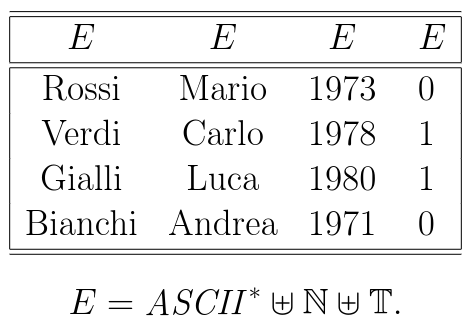
\includegraphics[width=\textwidth]{table.png}
    \caption{Esempio di relazione ordinata}
    \label{fig:tab}
\end{figure}

\subsubsection{Relazioni Non Ordinate}
Spesso conviene dare alle colonne di relazione un \textit{nome} e non solo una \textit{posizione}. Una relazione diventerebbe quindi: un insieme finito $\{f_1,...,f_n\}$ dove $f_i:C\to D$ e $C$ è un insieme finito di campi.

\bigskip

La nostra relazione d'esempio diventerebbe $\{f_1,f_2,f_3,f_4\}$ dove l'insieme $C$ è, per esempio \{COGNOME, NOME, ANNO, SOCIO\}.

\subsubsection{Equivalenza tra le due nozioni}
Ogni relazione \textbf{ordinata} può essere trasformata in una relazione \textbf{non ordinata} (è sufficiente \textit{dare un nome} a ciascun intero compreso tra 1 e $n$) e viceversa (basta fissare un \textit{ordine totale} su $C$).

\subsubsection{Query come funzioni}
Che funzione calcola una query? La base di dati è vista come una sequenza di relazioni, quindi il risultato deve essere anch'esso una relazione. In altre parole, la funzione $[Q]$ calcolata da una query $Q$ ha la forma seguente:

$[Q]:P_{fin}(D^{n_1})\times...\times P_{fin}(D^{n_k})\to P_{fin}(D^{n_m})$

\subsubsection{Algebra relazionale}
La sintassi dell'algebra relazionale sull'insieme dei simboli relazionali $\{R_1,...,R_k\}$ è la seguente:

\noindent$Q,P::= R_i\,\,|\,\,Q\cup P\,\,|\,\,Q-P\,\,|\,\,Q\times P\,\,|\,\,\pi_l(Q)\,\,|\,\,\sigma_c(Q)$\\
$c::= i\leq j\,\,|\,\,i=j\,\,|\,\,\lnot c\,\,|\,\,c\land d\,\,|\,\,c\lor d$
dove:
\begin{itemize}
    \item $i$ e $j$ sono numeri naturali positivi
    \item $l$ è la sequenza di numeri naturali positivi, ossia un elemento di $\mathbb{N}_+^*$
\end{itemize}
Un'interrogazione $Q$ soddisfa i \textbf{vincoli di integrità} se i numeri che occorrono in essa sono coerenti con la relazione a cui si riferiscono.

\bigskip

Data una query $Q$ su $\{R_1,...,R_k\}$, essa ha semantica:

\begin{center}
$[Q]:P_{fin}(D^{n_1})\times...\times P_{fin}(D^{n_k})\to P_{fin}(D^{n_m})$
\end{center}

dove $n_1,...,n_k$ sono le arietà di $R_1,...,R_k$ e $m$ è l'arietà di $Q$. La funzione $[Q]$ è definita per induzione sulla struttura di $Q$. Se $Q$ è $R_i$, allora $[Q](R_1,...,R_k)$ è semplicemente $R_i$. Gli operatori $\cup, -,\times$ hanno un'interpretazione insiemistica.

\bigskip

Nella proiezione, interviene una lista di interi $l$, che indica semplicemente quali campi considerare nella proiezione.
I vincoli d'integrità sono cruciali. Formalmente, $[\pi_{i_1,...,i_s}(Q)](R_1,...,R_k)$ sarà l'insieme

$\{(d_{i_1},...,d_{i_s})\,\,|\,\,(d_1,...,d_n)\in[Q](R_1,...,R_k)\}$

\bigskip

Nella selezione, interviene invece una condizione $c$, che indica quali tuple considerare nella selezione. I vincoli d'integrità sono cruciali. Data una tupla di valori $t=(d_1,...,d_n)$ e una condizione $c$, possiamo definire quando quest'ultima è soddisfatta in $(d_1,...,d_n)$, per induzione. La relazione $[\sigma_c(Q)](R_1,...,R_k)$ sarà

$\{t\,\,|\,\, t \in[Q](R_1,...,R_k)\land t\vdash c\}$


\subsubsection{Algebra relazionale - potere espressivo}
L'insieme delle funzioni che l'algebra relazionale ci permette di catturare sono quella della query ben formate:

$AR=\{[Q]\,\,|\,\,Q$ è una query ben formata\}

\subsubsection{Calcolo relazionale}
Un modo naturale per lavorare con le relazione è la logica predicativa. Supponiamo di voler interrogare una base di dati che consti delle relazioni $R_1,...,R_k$ aventi arietà $n_1,...,n_k$ ottenendo come \textbf{risultato} una relazione $Q$ di arietà $m$.

\bigskip

Basterà costruire una formula predicativa $F$ con:
\begin{itemize}
    \item Gli unici simboli funzionali sono delle \textit{costanti} che indicano gli elementi di $D$, mentre i simboli predicativi saranno $R_1,...,R_k$, più i simboli $\leq$ e $=$, questi ultimi preinterpretati
    \item Le variabili che occorrono libere in $F$ dovranno essere incluse nell'insieme $\{f_1,...,f_m\}$ e corrispondere ad un campo della relazione $Q$
\end{itemize}

Esempio:

\begin{table}[!ht]
    \centering
    \begin{tabular}{|ccccc|}
    \hline \hline
        0012 & Rossi & Mario & 1973 & 0 \\
        6783 & Verdi & Carlo & 1978 & 1 \\
        0987 & Gialli & Luca & 1980 & 1 \\
        4562 & Bianchi & Andrea & 1971 & 0 \\
        \hline\hline
    \end{tabular}
    \caption{Tabella $R_1$}
    \label{tab:r1}
\end{table}


\begin{table}[!ht]
    \centering
    \begin{tabular}{|cccc|}
    \hline \hline
        0012 & 6783 & 3 & 2 \\
        6783 & 4562 & 1 & 3 \\
        0987 & 4562 & 0 & 3 \\
        \hline\hline
    \end{tabular}
    \caption{Tabella $R_2$}
    \label{tab:r2}
\end{table}

Vogliamo trovare una formula per il calcolo relazione che catturi gli anni di nascita dei vincitori. Un esempio potrebbe essere:

\begin{center}
\noindent $\exists p.\exists s.\exists c.\exists n.\exists o.\exists pp.\exists ps.R_1(p,c,n,f,0)\land R_2(p,s,pp,ps)\land(pp>ps)$
\end{center}

\begin{center}
    $\lor$
\end{center}

\begin{center}
\noindent$\exists p.\exists s.\exists c.\exists n.\exists o.\exists pp.\exists ps.R_1(s,c,n,f,0)\land R_2(p,s,pp,ps)\land(ps>pp)$
\end{center}

\subsubsection{Calcolo relazione - semantica}
L'universo in cui \textit{interpretare} una formula $F$ del calcolo relazionale è $D$. Gli unici simboli che occorre \textit{interpretare} per dare una semantica a $F$ sono $R_1,...,R_k$. Quindi, è naturale vedere la base di dati $\{R_1,...,R_k\}$ come una tale interpretazione.

\bigskip

Se che vale che $(D,\{R_1,...,R_k\}),\xi\vDash F$, cioè significa che $(\xi(f_1),...,\xi(f_m))$ deve stare nella relazione $Q$.

\bigskip

Di conseguenza, possiamo porre $[F](R_1,...,R_k)$ pari a 

$\{(\xi(f_1),...,\xi(f_m))\,\,|\,\,(D,\{R_1,...,R_k\}),\xi\vDash F\}$

\bigskip

In questo modo, $[F]\subseteq D^m$, ma \textit{non è detto che $[F]$ sia finita!} Basti considerare la formula $F=(f_1=f_1)$.

\subsubsection{Calcolo relazione sicuro}
Occorre quindi isolare un sottoinsieme  delle formule del calcolo relazionale: le \textbf{formule sicure}. Se una formula $F$ è sicura, allora ogni tupla in $[F]$ contiene valori tra quelli che occorrono in $F$ e quelli che troviamo nelle tuple in $R_1,...,R_k$. Quindi, $[F]$ è sempre finita. Useremo l'insieme delle variabili che occorrono libere in una formula $F$, detto $FV(F)$.
\begin{enumerate}
    \item L'uso del quantificatore \textit{universale} non è permesso.
    \item Ogni volta che si utilizza l'operatore $\lor$ per formare $F\lor G$, deve valere che $FV(F) = FV(G)$.
    \item Se una sotto-formula della formula data di può scrivere come $F_1\land...\land F_m$, (dove $m\geq 1$ è massimale), allora ogni $x\in\cup_{1\leq i\leq m}FV(F_i)$ deve essere \textit{limitata}, ossia deve esistere \textit{almeno una} formula $F_j$ tale che:
    \begin{enumerate}
        \item $x\in FV(F_j)$ e $F_j$ non è un predicato aritmetico e non è nella forma $\lnot G$.
        \item $F_j$ è nella forma $x=c$ oppure $c=x$, dove $c$ è una costante.
        \item $F_j$ è nella forma $x=y$ dove $y$ è anch'essa limitata.
    \end{enumerate}
    \item L'unico uso permesso dell'operatore di negazione è in una delle formule $F_i =\lnot G$ di una congiunzione $F_1\land...\land F_m$ in cui vi sia almeno una delle $F_p$ che non sia essa stessa negata.
\end{enumerate}

\subsubsection{Calcolo Relazionale Sicuro - Potere Espressivo}
Definiamo l'insieme delle funzioni che il calcolo relazionale sicuro cattura:

\bigskip

$CR = \{[F]\,\,|\,\,F$ è una formula sicura del calcolo relazionale\}

\begin{quote}
    \textbf{Teorema:} $AR=CR$
\end{quote}

\textbf{Dimostrazione:} Passaggi principali:
\begin{enumerate}
    \item Dimostriamo prima $AR\subseteq CR$, la prova procede per induzione sulla struttura algebrica $A$ che vogliamo tradurre in $CR$
    \item occorre dire qualcosa sulle query di selezioni, definiamo \textbf{semplice} una query relazionale $Q$ tale che tutti gli operatori di selezione $\sigma_c(R)$ in $Q$ sono tali che $c$ è un operatore aritmetico o la sua negazione
    \item Lemma: per ogni $Q$ esiste $P$ semplice tale che $[Q]=[P]$. Per dimostrarlo, dimostriamo prima il seguente sottolemma per induzione su $c$: se $Q$ è semplice, allora esiste una query semplice $R$ equivalente a $\sigma_c(Q)$. Dato questo sottolemma, si dimostra il lemma per induzione su $Q$
    \item tornando a dimostrare $AR\subseteq CR$, procedendo per induzione su una query $Q$. Nel caso di $Q =\sigma_c(R)$ usiamo il lemma
    \item Ora dimostriamo $CR\subseteq AR$, per farlo passiamo per un linguaggio intermedio chiamato DATALOG. Un programma datalog ha forma $H:- B_1 \&...\& B_q$ dove $H$ è la testa della regola mentre $B$ è il corpo. La testa ha forma $P(A_1,...,A_n)$ dove $A$ sono variabili oppure costanti. Il corpo può avere predicati, relazioni, formule atomiche e operazioni logiche
    \item Per la prova ci interessa i programmi datalog non ricorsivi (bisogna controllare il grafo delle dipendenze) e sicuri (simile al $CR$ sicuro)
    \item Siamo interessati a dimostrare il seguente lemma: ogni programma datalog non ricorsivo e sicuro $D$ ha semantica ben definita
    \item Dobbiamo quindi trovare una funzione \verb|c2d| che traduca il $CR$ sicuro in datalog non ricorsivo e sicuro e una funzione \verb|d2a| che traduca a sua volta in $AR$: $F\to $\verb|c2a(c2d(|$F$\verb|))|
    \item la traduzione in datalog sarà definita per ricorsione sulla struttura $F$ (l'unica difficoltà è sul caso $F=G_1\land...\land G_m$)
    \item costruzione della funzione \verb|d2a|: si procederà attraverso 5 fasi
    \begin{enumerate}
        \item rettificazione delle regole
        \item calcolo dell'espressione dom
        \item calcolo dell'ordine topologico del grafo delle dipendenze
        \item calcolo di un'espressione dell'algebra relazionale per ciascuna regola del programma datalog
        \item calcolo di un'espressione dell'algebra relazionale per ciascuna relazione ausiliaria del programma datalog
    \end{enumerate}
    \item osserviamo coem sia stata fatta l'assuzione che la parte relazionale \textbf{NON} contenga costanti; tale assunzione non fa perdere generalità
\end{enumerate}

\subsection{Verifica dei sistemi e logica modulare}
Cosa significa verificare la correttezza di un sistema? Data la descrizione di un sistema $S$ e una proprietà $P$ che descriva il comportamento atteso, occorre \textbf{verificare} che $S$ effettivamente soddisfi $P$.

\bigskip

\'E possibile fare la verifica in modo automatico? Quasi sempre, lo scenario è il seguente: sia $S$ il programma da verificare e $P$ la proprietà da verificare. $A$ è il verificatore che darà un risposta $o\in\{yes, no, maybe\}$. Tra le possibili risposte c'è anche $maybe$ perché spesso verificare che $S$ soddisfi $P$ è spesso indecidibile (si potrà risolvere solo un'approssimazione del problema).

\subsubsection{Model Checking}
Nel model checking, si fa verifica considerando la proprietà $P$ come una formula di una opportuna logica e il sistema come un’interpretazione per essa.

\begin{figure}[!ht]
    \centering
    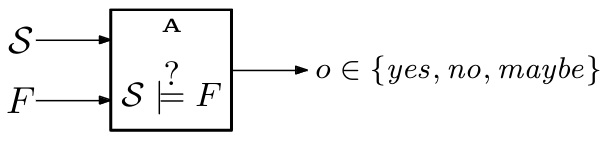
\includegraphics[width=\textwidth]{modelcheck.png}
    \caption{Concetto grafico di model checking}
    \label{fig:model}
\end{figure}

Bisogna però capire in che senso un sistema o programma possa essere visto come un'interpretazione e quale sia la logica adatta a specificare le proprietà d'interesse.

\subsubsection{Strutture di Kripke}
Supponiamo che $AP$ sia un insieme di proposizioni atomiche, che catturino le proprietà di interesse di uno stato, magari astraendo sullo stato stesso. Una \textbf{struttura di Kripke} su $AP$ è una quadrupla $M=(S,S_0,R,L)$ dove:
\begin{itemize}
    \item $S$ è un insieme di \textit{stati}.
    \item $S_0\subseteq S$ è l'insieme degli \textit{stati iniziali}
    \item $R\subseteq S\times S$ è la \textit{relazione di transizione}, che supponiamo totale: per ogni $s\in S$ esiste $t\in S$ con $(s,t)\in R$
    \item $L:S\to P(AP)$ è una \textit{funzione di etichettatura}
\end{itemize}

\bigskip

L'insieme degli strati si suppone spesso essere finito, questo per garantire la decidibilità. La funzione di etichettatura ha il ruolo di dire quale proposizione atomiche valgono in ogni stato. Vediamo un esempio.

\bigskip

Consideriamo il seguente programma \textit{concorrente}:

\bigskip

$(l_1:x\leftarrow0;l_2:y\leftarrow1)\,\,||\,\,(l_3:y\leftarrow0;l_4:x\leftarrow1)$

\bigskip

L'insieme degli \textit{stati} di questo programma può essere visto come l'insieme

\bigskip

$\{l_1,l_2,\cdot\}\times\{l_3,l_4,\cdot\}\times\{0,1\}\times\{0,1\}$

mentre l'unico stato iniziale potrebbe essere $(l_1,l_3,1,1)$.

\bigskip

La relazione di transizione corrisponde a quella intuitiva, ed è costruita usando il principio dell'\textit{interleaving}.

\begin{figure}[!ht]
    \centering
    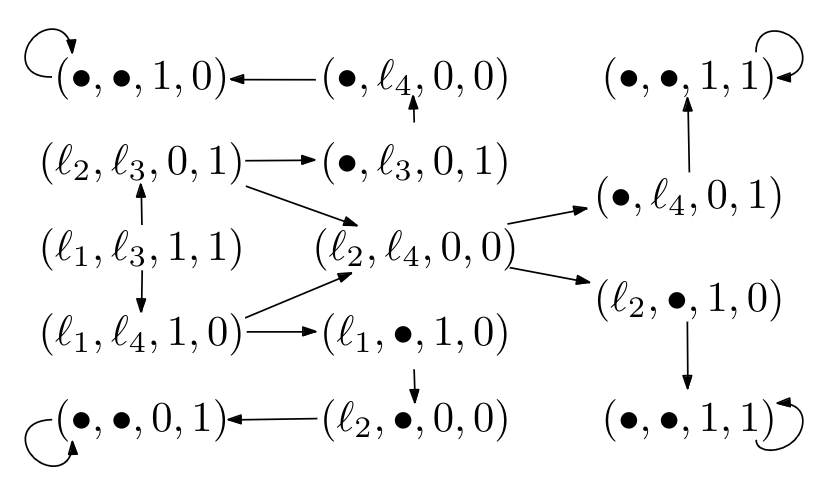
\includegraphics[width=\textwidth]{kripke.png}
    \caption{Sistema di transizione d'esempio}
    \label{fig:kripke}
\end{figure}

\bigskip

L'insieme $AP$ potrebbe contenere queste proposizioni: una chiamata \verb|null|, che modella il fatto che entrambe le variabili $x$ e $y$ valgono 0, e una chiamata \verb|stop|, che modella la terminazione del programma. Formalmente, \verb|null| $\in L(S)$ sse le ultime due componenti di $S$ sono entrambe 0; \verb|stop| $\in L(S)$ sse le prime due componenti di $S$ sono entrambe $\cdot$. Ciò non toglie che $AP$ possa contenere anche tante altre proposizioni atomiche, come per esempio $x=0,y=1,l_1$, il cui significato è intuitivo.

\bigskip

Come specificare proprietà di sistemi? Proviamo a sfruttare la \textbf{logica proposizionale} in cui le proposizioni atomiche sono gli atomi. In questo modo possiamo parlare del sistema in senso statico, ossia della struttura di Kripke e \textit{di un suo stato}.

\bigskip

Ad esempio, possiamo concludere che:

\begin{quote}
    $M,(l_1,l_3,0,0)\vDash$\verb| null|$\land\lnot$\verb|stop|
\end{quote}
\begin{quote}
    $M,(\cdot,\cdot,1,1)\vDash$\verb| null|$\to$\verb| stop|
\end{quote}

Si potrebbe scrivere $M\vDash F$ sse $M,S\vDash F$ per ogni $S\in S_0$.

\bigskip

Manca l'aspetto dinamico. Come esprimere proprietà relative all'\textbf{evoluzione} del sistema? Ad esempio: \textbf{reachability, safety}, etc...

\subsubsection{Logiche temporali}
Le logiche temporali possono essere viste come estensioni della logica proposizionale ottenute dotando quest'ultima di \textbf{operatori modali} che permettono di esprimere in che senso una formula vale \textit{nel futuro} e il fatto che certe formule valgano \textit{in alcune} esecuzioni nondeterministiche, oppure \textit{in tutte}.

\bigskip

\textbf{Operatori temporali}:
\begin{itemize}
    \item se una formula $F$ \textit{vale ora e rimane valida nel futuro}, allora scriviamo $(G\,\,F)$ dove $G$ sta per \verb|global|
    \item se una formula $F$ vale \textit{dopo la prossima} transizione di stato, allora scriviamo $(X\,\,F)$, dove $X$ sta per \verb|next|
    \item se una formula $D$ vale \textit{in un certo istante indefinito del futuro}, allora scriviamo $(F\,\,D)$ dove $F$ sta per \verb|future| 
\end{itemize}

\bigskip

\textbf{Quantificatori sui cammini}:  se una formula $F$ vale \textit{indipendentemente} dal nondeterminismo, allora scriveremo $(A\,\,F)$. Invece, se una formula $F$ vale per \textit{almeno una} scelta nondeterministica, allora scriveremo $(E\,\,F)$. $AP$ è un insieme di etichette (come \verb|null| e \verb|stop|).

\subsubsection{CTL$^*$}
La logica temporale CTL$^*$ descrive una logica che, grazie agli operatori temporali, produce formule da valutare su \textit{cammini} di esecuzione, mentre i quantificatori sui cammini vengono valutati su \textit{stati}.

\bigskip

\textbf{Formule di stato} su AP:
\begin{quote}
    $F_S,G_S::=P\,\,|\,\,F_S\land G_S\,\,|\,\,F_S\lor G_S\,\,|\,\,\lnot F_S\,\,|\,\,E\,\,F_P\,\,|\,\,A\,\,F_P$
\end{quote}
dove $P\in AP$.

\bigskip

\textbf{Formule di cammino} su AP:
\begin{quote}
    $F_P,G_P::=F_S\,\,|\,\,F_P\land G_P\,\,|\,\,F_P\lor G_P\,\,|\,\,\lnot G_P\,\,|\,\,X\,\,F_P\,\,|\,\,F\,\,F_P\,\,|\,\,G\,\,F_P\,\,|\\F_P\,\,U\,\,G_P\,\,|\,\,F_P\,\,R\,\,G_P$
\end{quote}

\bigskip

Definiamo la \textit{semantica} della logica temporale. Un \textbf{cammino} $\pi$ in una struttura di Kripke $M=(S,S_0,R,L)$ è una sequenza infinita di stati $s_0s_1s_2...\in S^\omega$ tale che $(s_n,s_{n+1})\in R$ per ogni naturale $n$.

\bigskip

Dato un cammino $\pi$ e un naturale $n$, indicheremo con $\pi^n$ l'$n$-esimo suffisso di $\pi$, anch'esso cammino. Una formula di stato $F_S$ su $AP$ è vera in una struttura di Kripke $M$ su $AP$ e in uno stato $s$ di $M$. In tal caso scriveremo $M,s\vDash F_s$.

\bigskip

Una formula di cammino $F_P$ su $AP$ è vera in una struttura di Kripke $M$ su $AP$ e in un cammino $\pi$ in $M$. In tal caso scriveremo $M,\pi\vDash F_P$.

\bigskip

Per quanto riguarda le formule di stato, i connettivi $\lnot, \land$ e $\lor$ sono interpretati in modo standard. Le proposizioni atomiche si interpretano facendo riferimento alla struttura di Kripke: $(S,S_0,R,L),s\vDash P$ sse $P\in L(s)$. I quantificatori sui cammini fanno riferimento alla semantica delle formule di cammino:
\begin{itemize}
    \item $M,s\vDash (E\,\,F_P)$ sse $M,\pi\vDash F_P$ per almeno un cammino $\pi$ che inizi in $s$
    \item $M,s\vDash (A\,\,F_P)$ sse $M,\pi\vDash F_P$ per tutti i cammini $\pi$ che inizi in $s$
\end{itemize}

Per quanto riguarda le formule di cammino, i connettivi $\lnot, \land$ e $\lor$ sono interpretati in modo standard. Le formule di stato si valutano nel primo stato di cammino $F,\pi\vDash F_S$ sse $F,s\vDash F_S$. I quantificatori sui cammini fanno riferimento alla semantica delle formule di cammino:
\begin{itemize}
    \item $M,\pi\vDash(X\,\,F_P)$ sse $M,\pi^1\vDash F_P$
    \item $M,\pi\vDash(F\,\,F_P)$ sse $M,\pi^i\vDash F_P$ per almeno un $i$
    \item $M,\pi\vDash(G\,\,F_P)$ sse $M,\pi^i\vDash F_P$ per tutti gli $i$
    \item $M,\pi\vDash(F_P\,\,U\,\,G_P)$ sse esiste $k$ naturale con $M,\pi^k\vDash G_P$ e $M,\pi^j\vDash F_P$ per ogni $0\leq j\leq k$
    \item $M,\pi\vDash(F_P\,\,R\,\,G_P)$ sse per ogni $j$ naturale, se per ogni $i<j,M,\pi^i\not\vDash F_P$, allora $M,\pi^j\vDash G_P$
\end{itemize}

\subsubsection{Frammenti di CTL$^*$}
Logica CTL:
\begin{itemize}
    \item ogni operatore temporale deve essere immediatamente preceduto da un quantificatore sui cammini
    \item la grammatica per le formule di cammino diventa molto più semplice
    \begin{quote}
        $F_P,G_P::= X\,\,F_S\,\,|\,\,F\,\,F_S\,\,|\,\,G\,\,F_S\,\,|\,\,F_S\,\,U\,\,G_S\,\,|\,\,F_S\,\,R\,\,G_S$
    \end{quote}
\end{itemize}

\noindent Logica LTL:
\begin{itemize}
    \item le uniche formule considerate sono le formule di cammino, che però vengono implicitamente quantificate con il quantificatore $A\cdot$
    \item le formule diventano
    \begin{quote}
        $F_P,G_P::=P\,\,|\,\,F_P\land G_P\,\,|\,\,F_P\lor G_P\,\,|\,\,\lnot G_P\,\,|\,\,X\,\,F_P\,\,|\,\,F\,\,F_P\,\,|\,\,G\,\,F_P\,\,|\\F_P\,\,U\,\,G_P\,\,|\,\,F_P\,\,R\,\,G_P$
    \end{quote}
\end{itemize}

\subsubsection{Il problema del model checking}
\textbf{Model Checking Universale}: data un struttura di Kripke $M$ e una formula di $F_S$, determinare se $M,s \vDash F_S$ per ogni $s\in S_0$.

\bigskip

\noindent\textbf{Model Checking Esistenziale}: data un struttura di Kripke $M$ e una formula di $F_S$, determinare se esiste $s\in S_0$ con $M,s \vDash F_S$.

\begin{quote}
    \textbf{Teorema:} i problemi del model checking universale e esistenziale sono $PSPACE$-completi per CTL$^*$
\end{quote}

\textbf{Dimostrazione:} non data.

\begin{quote}
    \textbf{Teorema:} i problemi del model checking universale e esistenziale per CTL sono risolvibili in tempo polinomiale.
\end{quote}

\textbf{Dimostrazione:} Passaggi principali:
\begin{enumerate}
    \item Grazie a dei lemmi possiamo assumere che la formula su ciò si voglia fare model checking contenga solo $EX, EG, EU$ oltre agli operatori booleani
    \item costruiamo un algoritmo che risolve il model checking in CTL
    \item per l'algoritmo ci sarà bisogno di due procedure ausiliarie chiamate \verb|CheckEU| e \verb|CheckEG|
    \item l'algoritmo di \verb|CheckEU| procederà costruendo l'insieme degli stati che soddisfano $E(H\,\,U\,\,K)$ in un determinato modo
    \item l'algoritmo \verb|CheckEG| ha come idea cruciale, quella di utilizzare il concetto di componente fortemente connesso (SCC) di un grafo, ossia un sottoinsieme $P$ dei nodi del grafo tale per cui ogni elemento di $P$ sia raggiungibile da qualunque altro elemento di $P$
    \item bisogna dimostrare il seguente lemma: $M,S\vDash EG\,\,F$ sse è possibile costruire un cammino che da $s$ porti, tramite $R$ ad una SCC (massimale e non triviale) contenente stati che soddisfino $F$
    \item dimostrando il lemma è quello che serve per costruire \verb|CheckEG|, il quale procederà determinando le SCC massimali e nontriviali di $M$ che contengono solo stati in \verb|States[F]|, per poi controllare da quali stati in \verb|States[F]| tali SCC siano raggiungibili
\end{enumerate}



\subsubsection{Esempi di logica modale}

\begin{figure}[!ht]
    \centering
    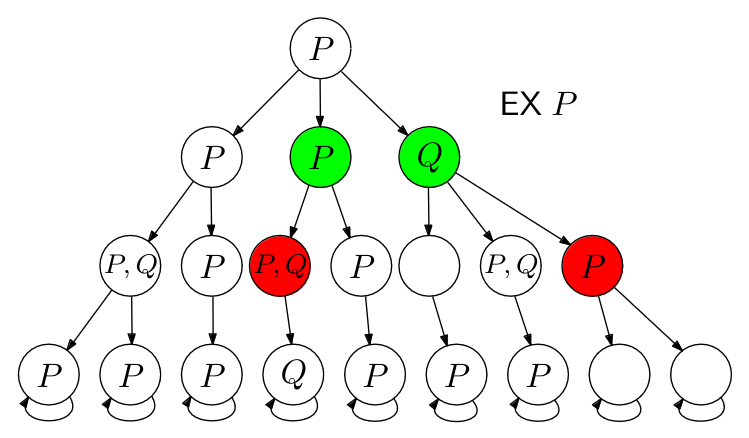
\includegraphics[width=0.6\textwidth]{exp.png}
    \caption{Esempio di logica modale per $EX\,\, P$}
    \label{fig:exp}
\end{figure}


\begin{figure}[!ht]
    \centering
    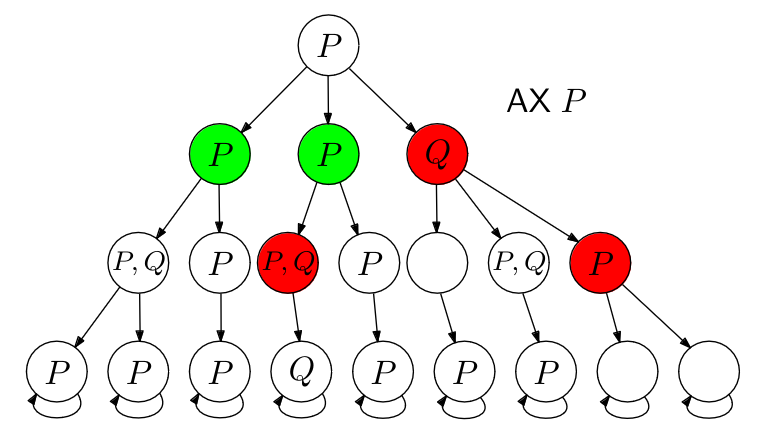
\includegraphics[width=0.6\textwidth]{axp.png}
    \caption{Esempio di logica modale per $AX\,\, P$}
    \label{fig:exp}
\end{figure}


\begin{figure}[!ht]
    \centering
    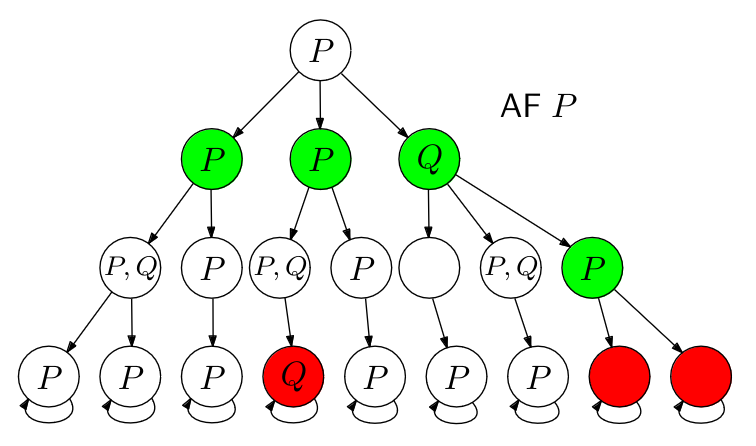
\includegraphics[width=0.6\textwidth]{afp.png}
    \caption{Esempio di logica modale per $AF\,\, P$}
    \label{fig:exp}
\end{figure}


\begin{figure}[!ht]
    \centering
    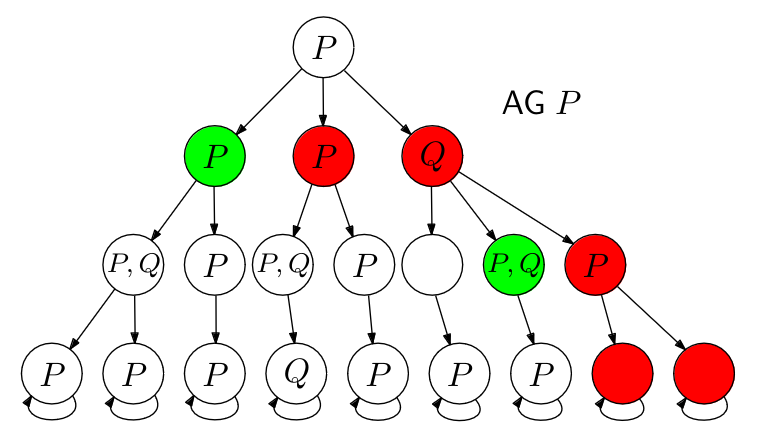
\includegraphics[width=0.6\textwidth]{agp.png}
    \caption{Esempio di logica modale per $AG\,\, P$}
    \label{fig:exp}
\end{figure}


\begin{figure}[!ht]
    \centering
    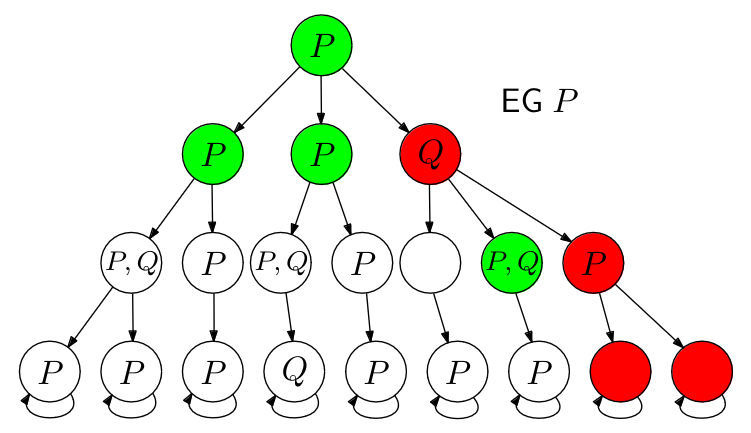
\includegraphics[width=0.6\textwidth]{egp.png}
    \caption{Esempio di logica modale per $EG\,\, P$}
    \label{fig:exp}
\end{figure}


\begin{figure}[!ht]
    \centering
    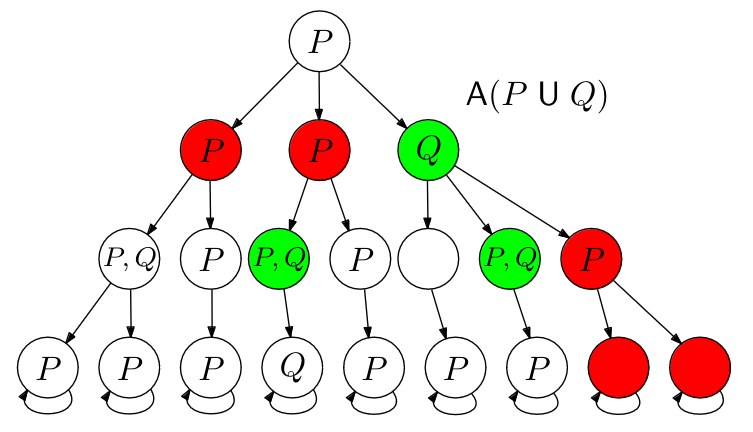
\includegraphics[width=0.6\textwidth]{apuq.png}
    \caption{Esempio di logica modale per $A(P\,\,U\,\,Q)$}
    \label{fig:exp}
\end{figure}


\begin{figure}[!ht]
    \centering
    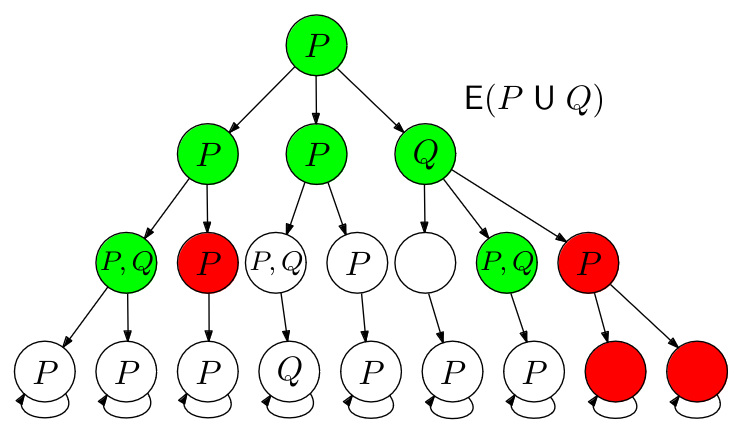
\includegraphics[width=0.6\textwidth]{epuq.png}
    \caption{Esempio di logica modale per $E(P\,\,U\,\,Q)$}
    \label{fig:exp}
\end{figure}


\newpage

\subsubsection{Esempi di logica modale con formule}

Primo esempio. Abbiamo un sistema che riceve richieste che deve poi soddisfare. Definiamo le variabili proposizionali:
\begin{quote}
    \verb|requested[i]| con $i\in\{1,...,n\}$ vuol dire che nello stato corrente ho ricevuto la richiesta $i$
\end{quote}
\begin{quote}
    \verb|acknowledged[i]| con $i\in\{1,...,n\}$ vuol dire che nello stato corrente la $i$-esima richiesta è stata soddisfatta
\end{quote}

\bigskip 

Se vogliamo dire che ogni richiesta, se ricevuta, verrà soddisfatta prima o poi, possiamo scrivere il seguente statement:
\begin{quote}
    $\land_{i=1}^n A\,G\,\,($\verb|requested[i]|$\to A\,F\,\,$\verb|acknowledged[i]|$))$
\end{quote}

\bigskip

Secondo esempio. Stiamo cercando di verificare il sistema di controllo di un ascensore. Definiamo le variabili proposizionali:
\begin{quote}
    \verb|floor[i]| con $i\in\{1,...,n\}$ vuol dire che l'ascensore è al piano $i$
\end{quote}
\begin{quote}
    \verb|direction[d]| con $d\in\{up,down\}$ indica la direzione dell'ascensore
\end{quote}
\begin{quote}
    \verb|buttonpressed[i]| con $i\in\{1,...,n\}$ vuol dire che il bottone del piano $i$-esimo è premuto
\end{quote}

\bigskip

Se un ascensore sta salendo e si trova in un piano inferiore al quinto, mentre il pulsante del quinto piano è premuto, l'ascensore deve continuare a salire finché non raggiunge il quinto piano.
\begin{quote}
$\land_{i=1}^4(($\verb|floor[i]| $\land$ \verb|direction[up]| $\land$ \verb|buttonpressed[5]|$)\to \\ A($\verb|direction[up] |$\cup$\verb| floor[5]|$))$
\end{quote}

\bigskip

Terzo esempio. Abbiamo a che fare con un sistema di allarme che segnala la presenza di eventi anomali con certe garanzie temporali. Definiamo 4 atomi proposizionali: 2 per i sensori (\verb|intrusion| e \verb|lowbattery|) e 2 per gli attuatori (\verb|alarm| e \verb|signal|).

\bigskip

Vorremmo essere sicuri che, se viene rilevata un'intrusione, scatti l'allarme entro 3 istanti:
\begin{quote}
    $A\,G\,\,($\verb|intrusion|$\to[AX(AX(AX($\verb|alarm|$)))\lor$\\$AX(AX($\verb|alarm|$))\lor$\\$AX($\verb|alarm|$)\lor$\\ \verb|alarm|$])$
\end{quote}

\bigskip

Inoltre, se c'è il rischio di rilevare un basso livello di batteria nei prossimi $n$ istanti, occorre segnalarlo immediatamente e per almeno 2 istanti. Definiamo la formula $EX^nF$ per induzione su $n$:

$EX^0F\equiv F$

$EX^{n+1}F\equiv F\lor EX(EX^nF)$

\bigskip

In questo modo abbiamo che la formula $EX^n$\verb|lowbattery| cattura proprio il rischio che in $n$ passi il sistema si possa trovare in una situazione di batteria scarica. Quindi possiamo scrivere la specifica:
\begin{quote}
    $A\,G\,\,[EX^n$ \verb|lowbattery|$\to$\verb|signal|$\lor AX($\verb|signal|$)\lor AX(AX($\verb|signal|$))]$
\end{quote}



\end{document}
